\documentclass[a4paper,12pt]{article}

\usepackage{geometry}
\geometry{top=15mm}
\geometry{bottom=30mm}
\geometry{left=10mm}
\geometry{right=20mm}
\linespread{1}
\setlength{\parindent}{12pt}
\setlength{\parskip}{8pt}

\usepackage{titleps}

\newpagestyle{main}
{
  \setheadrule{0.4pt}
  \sethead{}{}{}
  \setfootrule{0,4pt}
  \setfoot{}{\thepage}{}
}
\usepackage{color}
\usepackage[english,russian]{babel}
\usepackage[T2A]{fontenc}
\usepackage[utf8]{inputenc}
\usepackage{amsthm,amsmath,amsfonts,amssymb,mathtools}
\usepackage{indentfirst}
\usepackage{lipsum}
\usepackage{graphicx}
\usepackage{float}
\usepackage{wrapfig}

\newcommand{\partdef}[2]{\frac{\partial \mathnormal{#1}}{\partial \mathnormal{#2}}}

\begin{document}


\section*{Теоретическое решение дифференциального уравнения.}


\subsection*{Линейная задача.}
Решаем уравнение $u_t+\frac{u_x}{2}=0$, с начальными условиями
\begin{align*}
u_0(x)=\left\{
    \begin{array}{l}
        $0 \text{ , если } х \leqslant 0$
        \\
        $1 \text{ , если } х > 0$
    \end{array}
\right. 
\end{align*}
Запишем характеристическую систему уравнений:
\begin{align*}
\left\{
    \begin{array}{l}
        \dot t=1
        \\
        \dot x=\frac{1}{2}
    \end{array}
\right.   \Rightarrow  2x-t=const - \text{уравнение характеристик.}
\end{align*}
Вспомним \textbf{ утверждение :}\newline
$u -$ решение дифференциального уравнения $\Longleftrightarrow u -$ первый интеграл системы характеристик.

Иначе говоря, общее решение уравнения примет вид: $u=f(2x-t)$.
С учетом начальных условий имеем разрывное решение (см. рис. 1) 
$u(t,x)=\left\{
    \begin{array}{l}
        $1 \text{ , если } \{t > 0\}\cap\{2x -t > 0\}$
        \\
        $0 \text{ , если } \{t > 0\}\cap\{2x - t \leqslant 0\}$
    \end{array}
\right.$

\subsection*{Нелинейная задача.}
Решаем уравнение $u_t+u\cdot u_x=0$, с теми же начальными условиями.
Запишем характеристическую систему уравнений:
\begin{align*}
\left\{
    \begin{array}{l}
        \dot t=1
        \\
        \dot x=u
        \\
        \dot u=0
    \end{array}
\right.   \Rightarrow  x = u_0 t+x_0 - \text{уравнение характеристик.}
\end{align*}

Видим, что имеется область $\Omega$  (см. рис. 2), которая не покрывается характеристиками, поэтому в этой области ищется автомодельное решение $u=v(\frac{x}{t})$, что приводит к  $v(\frac{x}{t})=\frac{x}{t}$.

Таким образом получаем решение, суть которого передана рисунком 3.
\begin{figure}[h]
    \begin{center}
    \begin{minipage}[h]{0.3\linewidth}
    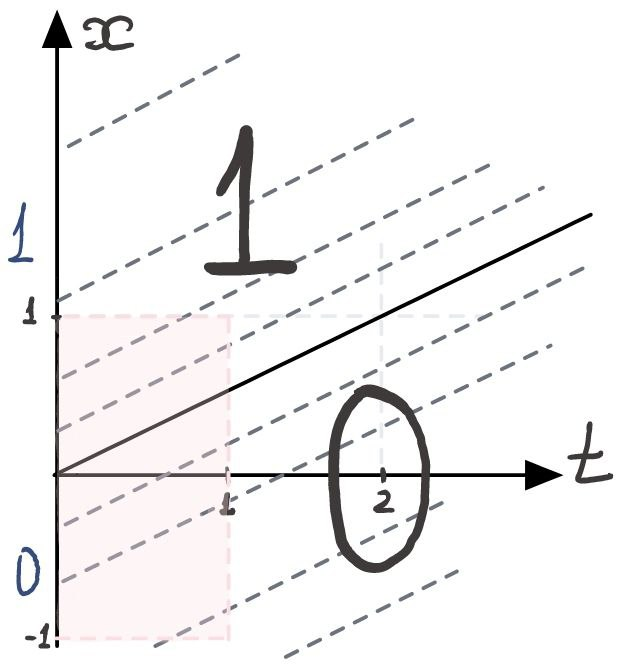
\includegraphics[width=0.8\linewidth]{photo1.jpg}
    \caption{}
    \end{minipage}
    \hfill
    \begin{minipage}[h]{0.3\linewidth}
    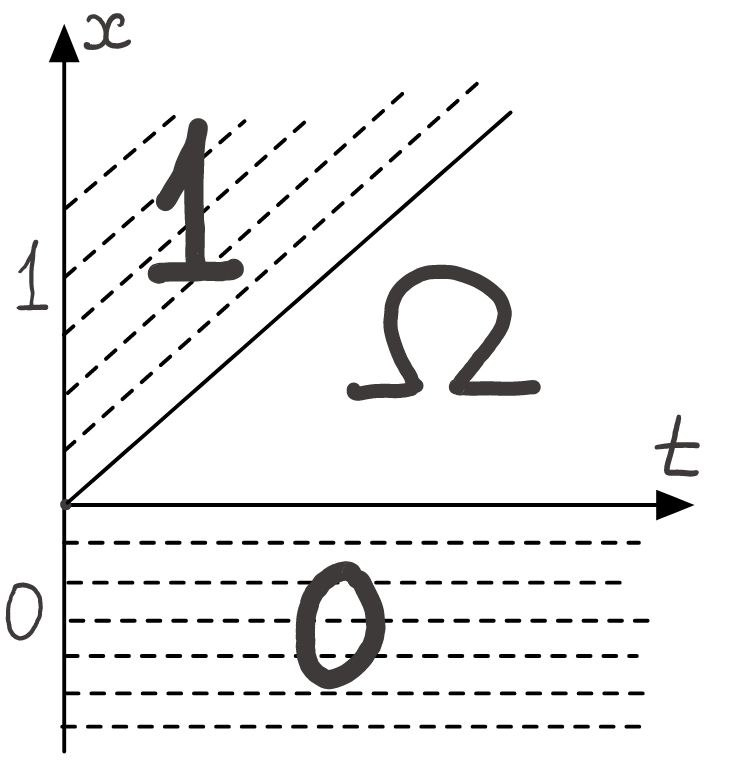
\includegraphics[width=0.8\linewidth]{photo2.jpg}
    \caption{}
    \end{minipage}
    \hfill
    \begin{minipage}[h]{0.3\linewidth}
    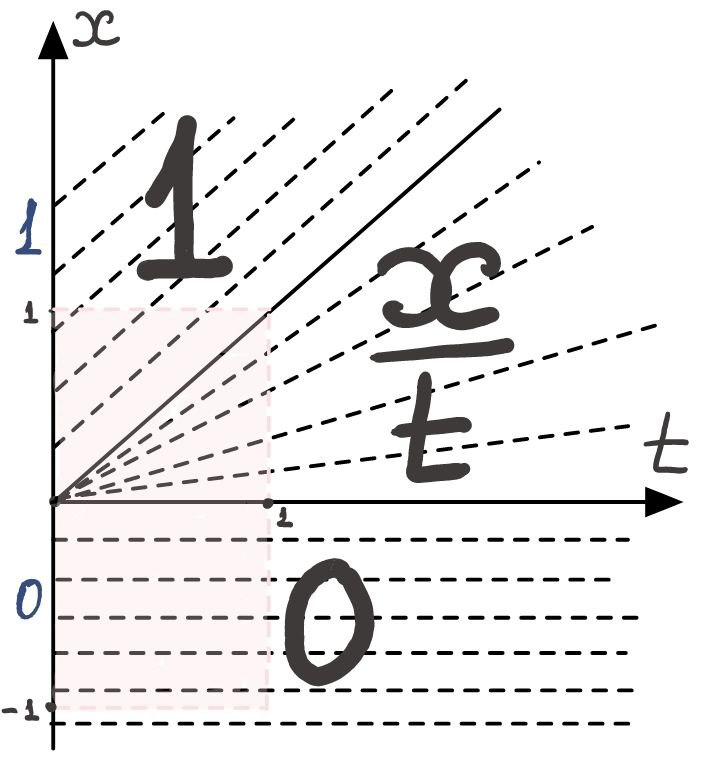
\includegraphics[width=0.8\linewidth]{photo3.jpg}
    \caption{}
    \end{minipage}    
    \end{center}
\end{figure}

\newpage
\section{Линейная задача.}
Итак, решаем $v_t+\frac{v_x}2=0$ в области $Q_T=\{(t,x)|0<t\leqslant 1, -1\leqslant x\leqslant 1 \}=\{(k_1 \tau,k_2 h),k_1 \in (0 \div N),k_2 \in(0 \div M_h)\}$. Начальные условия $v_0(x)=\left\{
\begin{array}{l}
        $0 \text{ , если } х \leqslant 0$
        \\
        $1 \text{ , если } х > 0$
\end{array}
\right.$. Из теоретического решения знаем, что граничные условия примут вид: $v(t,1)=1$ ,$v(t,-1)=0$
\subsection{Явная схема.}
\[
    v_m^{(1)}=v_m^n-\frac{\tau}{h}(F^n_{m+1}-F^n_m);\;\; v^{n+1}_m=\frac12\left(v^n_m+v_m^{(1)}-\frac{\tau}{h}(F(v_m^{(1)})-F(v_{m-1}^{(1)}))\right)
\]
из чего получаем разностную схему ($F(v)=\frac{v}{2}$)
\[
    S:=\frac{v^{n+1}_m-v^n_m}{\tau}+\frac{v^n_{m+1}-v^n_m}{4h}+\frac{v^{(1)}_m-v^{(1)}_{m-1}}{4h}=0
\]    
\subsubsection{Аппроксимация}
Используя выражения
\begin{align*}
\begin{array}{l}
    v_m^{n+1}=v+\dot v \tau+\frac{\ddot v}{2} {\tau}^2+\frac{\dddot v}6{\tau}^3+O({\tau}^4)\\
    v_m^n=v\\
    v^n_{m+1}=v+v' h+\frac{v''}2 h^2+\frac{v'''}6 h^3 +O(h^4)\\
    v^n_{m-1}=v-v' h+\frac{v''}2 h^2-\frac{v'''}6 h^3 +O(h^4)\\
    v_m^{(1)}=v_m^n-\frac{\tau}{2h}(v^n_{m+1}-v^n_m)\\
    v_{m-1}^{(1)}=v_{m-1}^n-\frac{\tau}{2h}(v^n_m-v^n_{m-1})\\
    \\
    \dot v +\frac12v'=0\\
    \ddot v-\frac14v''=0
\end{array}
\end{align*}
Получим 
\[S=\frac{\dddot v}6 {\tau}^2+\frac{v'''}{12} h^2+O(\tau^3+h^3)\]
Из чего делаем вывод, что порядок аппроксимации равен 2-ум. 
\subsubsection{Дифференциальное приближение}
\[
0=\dot v + \frac{v'}{2} + \frac{\tau}{2}(\ddot v - \frac{v''}{4}) + \frac{\dddot v}{6}{\tau}^2 +\frac{v'''}{12}h^2+O(\tau^3+h^3)
\]
\[
\dot v + \frac{v'}{2} = -\frac{\tau}{2}(\ddot v - \frac{v''}{4}) - \frac{\dddot v}{6}{\tau}^2 -\frac{v'''}{12}h^2+O(\tau^3+h^3)
\]
\begin{align*}
\left\{
\begin{array}{l}
\ddot v+ \frac{\dot v'}{2}=-\frac{\tau}{2}(\dddot v - \frac{\dot v''}{4})+O(\tau^2+h^2)\\
\\
\dot v'+\frac{v''}{2}=-\frac{\tau}{2}(\ddot v'-\frac{v'''}{4})+O(\tau^2+h^2)
\end{array} \Rightarrow \ddot v=\frac{v''}{4}-\frac{\tau}{2}(\dddot v -\frac{\dot v''}{4}-\frac{\ddot v'}{2}+\frac{v'''}{8})+O(\tau^2+h^2)
\end{align*}
\[
\dot v+\frac{v'}{2}=\frac{\dddot v}{12}\tau^2-\frac{\dot v''}{16}\tau^2-\frac{\ddot v'}{8}\tau^2+\frac{v'''}{32} \tau^2-\frac{v'''}{12}h^2+O(\tau^3+h^3)
\]
\begin{align*}
\left\{
\begin{array}{l}
\dddot v=\frac{\dot v''}{4}+O(\tau+h)\\
\\
\dot v''=-\frac{v'''}{2}+O(\tau+h)\\
\\
\ddot v'=-\frac{\dot v''}{2}+O(\tau +h)
\end{array}\Rightarrow
\begin{array}{l}
\dddot v=-\frac{v'''}{8}+O(\tau+h)\\
\\
\dot v''=-\frac{v'''}{2}+O(\tau+h)\\
\\
\ddot v'=\frac{v'''}{4}+O(\tau +h)
\end{array} \Rightarrow
\end{align*}
\[
\Rightarrow    \dot v+\frac{v'}{2}=\frac{v'''}{48}(\tau^2-4h^2)+O(\tau^3+h^3)
\]
\subsubsection{Спектральная устойчивость.}
При замене $v^n_m=\lambda^n e^{i m \varphi}$ получаем ($\nu = \frac{\tau}h$) :

$\lambda(\varphi)=1+\frac{\nu^2}{4} \cos{\varphi}-\frac{\nu^2}{4} - \frac{\nu}{2} \sin{\varphi}\; i$ , положим $\lambda = x+i\; y$ , тогда 

\[
    \frac{16(x-1+\frac{\nu^2}{4})^2}{\nu^4}+\frac{4 \; y^2}{\nu^2} \;=\;1
\] - что является эллипсом, правый край которого лежит в точке (0.1). Заметим, что левый край эллипса, лежащий в точке $(1-\frac{\nu^2}{2},0)$ , находится внутри окружности радиуса 1. Из геометричесских свойств эллипса и окружности, чтобы эллипс целиком лежал в единичной окружности, достаточно того, что в точке касания эллипса и окружности, эллипс оказался "вогнутее" окружности. Выразим для этого правые половины фигур, как функции переменной $y$ ($x_1(y)$ - окружность, $x_2(y)$ - эллипс.),  и разложим их в ряд Тейлора в нуле. Получим: 

$
x_1(y)=1-\frac{y^2}{2}-\frac{y^4}{8}+O(y^6) ,
$

$
x_2(y)=1-\frac{y^2}{2}-\frac{y^4}{2\; \nu^2}+O(y^6).
$ 

Откуда видно, что при ограничении $\nu\;<\;2$ желаемое выполнено, а значит эллипс лежит целиком в единичной окружности. При $\nu\;=\;2$ эллипс совпадет с окружностью.

Итак, при $\nu\leqslant\;2$ имеем $max_{\varphi}|\lambda(\varphi)|\leqslant 1$. При $\nu>2\;:\;max_{\varphi}|\lambda(\varphi)|=2 \nu -1$. Необходимо выполнение $2 \nu -1 \leqslant 1 + C \tau \;\;\Rightarrow\;\; C \geqslant \frac{2(\tau-h)}{\tau h}\;\geqslant\;\frac{2}{\tau}$ - что противоречит независимости константы С от параметров сетки. 

Таким образом доказали, что при $\nu\leqslant\;2$ имеем условную спектральную устойчивость.

\subsubsection{Численное решение задачи.}
Граничные условия примут вид: $v(t,-1)=0 \Rightarrow v^n_0=0 \;\; \forall\; n \in (0 \div N)$ , $v(t,1)=1 \Rightarrow v^n_{M_h}=0 \;\; \forall\; n \in (0 \div N)$.

Тогда  $\{v^{n+1}_m\}$ считается по набору $\{v^{n}_m\}$ согласно системе линейных уравнений:
\[
    v^{n+1}_m=v^n_m-\frac{\nu}{4}(v^n_{m+1}-v^n_{m-1})+\frac{{\nu}^2}{8} ( v^n_{m+1}-2 v^n_m + v^n_{m-1})\text{,  где $m \in (1 \div M_h-1)$.}
\]

Тогда расчеты дают следующие результаты:
\begin{align*}
\begin{tabular}{|c|c|c|c|c|c|}
    \hline
    \tau & h & \Delta(v)_{C_h} & \Delta(v)_{L_1,h} & \delta(v)_{C_h} & \delta(v)_{L_1,h} \\
    \hline
    0.100 & 0.100 & 4.562959e-01 & 1.165588e-01 & 4.562959e-01 & 2.087832e-01 \\
    \hline
    0.010 & 0.100 & 5.235515e-01 & 2.231802e-01 & 5.235515e-01 & 3.388837e-01 \\
    \hline
    0.001 & 0.100 & 5.281042e-01 & 2.518680e-01 & 5.281042e-01 & 3.664916e-01 \\
    \hline
    0.100 & 0.010 & 7.079067e+15 & 3.989613e+14 & 1.000000e+00 & 1.000000e+00 \\
    \hline
    0.010 & 0.010 & 5.758615e-01 & 2.985708e-02 & 5.758615e-01 & 5.782227e-02 \\
    \hline
    0.001 & 0.010 & 6.024730e-01 & 5.499514e-02 & 6.024730e-01 & 1.018212e-01 \\
    \hline
    0.100 & 0.001 & 8.667438e+35 & 4.873056e+33 & 1.000000e+00 & 1.000000e+00 \\
    \hline
    0.010 & 0.001 & 2.953740e+167 & 5.230919e+165 & 1.000000e+00 & 1.000000e+00\\ 
    \hline
    0.001 & 0.001 & 6.263008e-01 & 7.563841e-03 & 6.263008e-01 & 1.498940e-02\\ 
    \hline
\end{tabular}
\end{align*}

Теперь рассмотрим случай равномерного дробления сетки, при исходных данных $\tau = 0.1$, $h = 0.1$.
Причем $\tau_k=\frac{\tau}{2^k}$ и $h_k=\frac{h}{2^k}$.  $\Delta(v,v^k)_\alpha=\|v-v^k\|_\alpha$  и  $\delta(v,v^k)_\alpha=\frac{\|v-v^k\|_\alpha}{\|v\|_{\alpha}}$. 
\begin{align*}
\begin{tabular}{|c|c|c|c|c|c|c|}
    \hline
     & \tau_k& h_k & \Delta(v,\cdot)_{C_h} & \Delta(v,\cdot)_{L_1,h} & \delta(v,\cdot)_{C_h} & \delta(v,\cdot)_{L_1,h} \\   
    \hline
   v^1 & 0.050000 & 0.050000 & 1.623536e-01 & 7.117751e-02 & 1.623536e-01 & 1.274951e-01 \\
   \hline
   v^2 & 0.025000 & 0.025000 & 2.538785e-01 & 1.031411e-01 & 2.538785e-01 & 1.847491e-01 \\
   \hline
   v^3 & 0.012500 & 0.012500 & 2.172151e-01 & 8.127450e-02 & 2.172151e-01 & 1.455811e-01 \\
   \hline
   v^4 & 0.006250 & 0.006250 & 2.190073e-01 & 8.846131e-02 & 2.190073e-01 & 1.584543e-01 \\
   \hline
   u & 0.100000 & 0.100000 & 4.562959e-01 & 1.165588e-01 & 4.562959e-01 & 2.087832e-01 \\
    \hline
\end{tabular}
\end{align*}
    
При исходных данных $\tau = 0.01$, $h = 0.01$.
\begin{align*}
\begin{tabular}{|c|c|c|c|c|c|c|}
    \hline
     & \tau_k& h_k & \Delta(v,\cdot)_{C_h} & \Delta(v,\cdot)_{L_1,h} & \delta(v,\cdot)_{C_h} & \delta(v,\cdot)_{L_1,h} \\   
    \hline
    v^1 & 0.005000 & 0.005000 & 2.872700e-01 & 2.038365e-02 & 2.872700e-01 & 3.947568e-02\\ 
    \hline
    v^2 & 0.002500 & 0.002500 & 4.182928e-01 & 2.551242e-02 & 4.182928e-01 & 4.940824e-02\\
    \hline
    v^3 & 0.001250 & 0.001250 & 4.969920e-01 & 2.570726e-02 & 4.969920e-01 & 4.978559e-02\\ 
    \hline
    v^4 & 0.000625 & 0.000625 & 6.390749e-01 & 2.660494e-02 & 6.390749e-01 & 5.152407e-02\\ 
    \hline
    u & 0.010000 & 0.010000 & 5.758615e-01 & 2.985708e-02 & 5.758615e-01 & 5.782227e-02\\
    \hline
\end{tabular}
\end{align*}

Таким образом имеем следующие графики:
\begin{figure}[h]
    \begin{center}
    \begin{minipage}[h]{0.42\linewidth}
    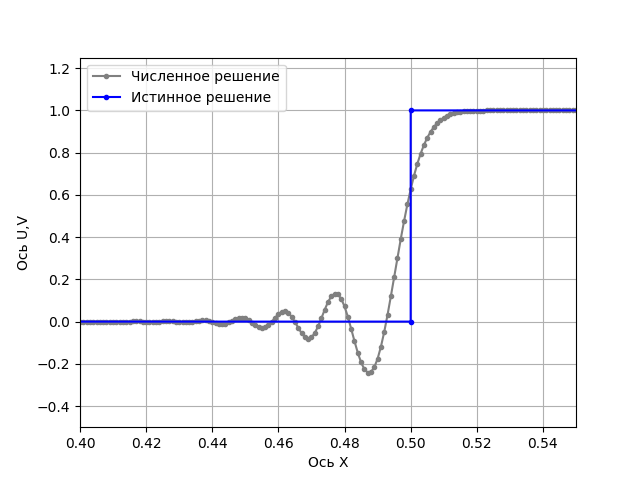
\includegraphics[width=1\linewidth]{Figure_1.png}
    \end{minipage}
    \hfill
    \begin{minipage}[h]{0.57\linewidth}
    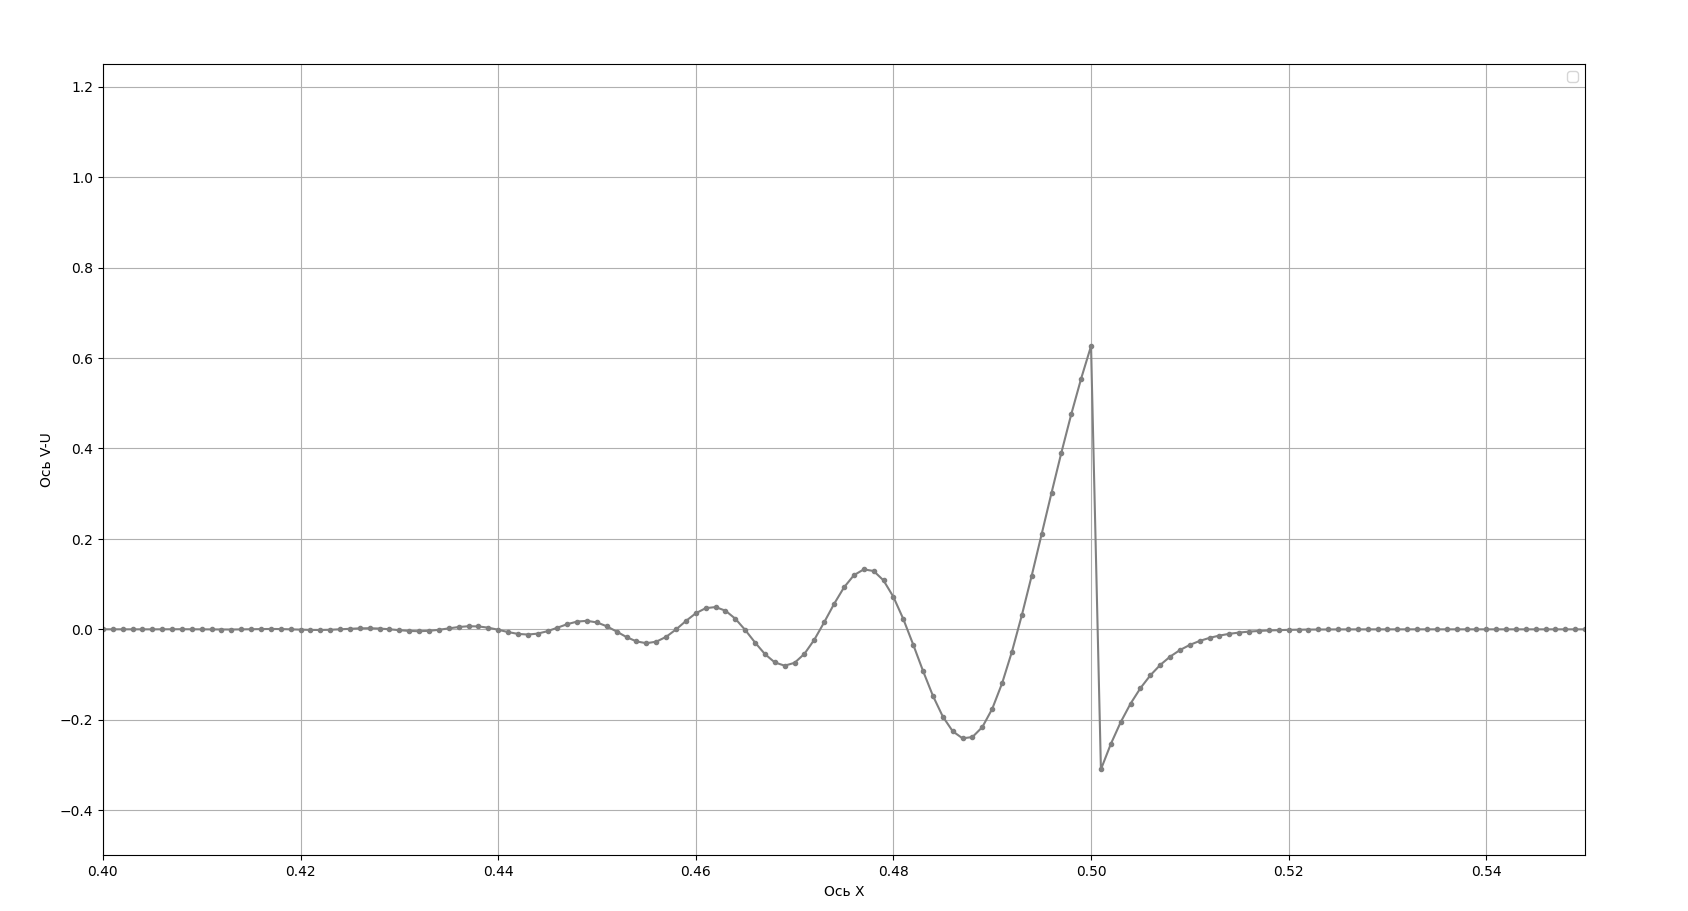
\includegraphics[width=1\linewidth]{Figure_2.png}
    \end{minipage}
    \hfill
    \end{center}
\end{figure}

\subsection{Неявная схема.}
\[
   S:=v_t+\frac12 (F(\hat{v}))_x+\frac12 (F(v))_\overline{x}=0 
\]
Схема примет вид $(F(v)=\frac{v}{2})$:
\[
S=\frac{v^{n+1}_m-v^n_m}{\tau}+\frac{v^{n+1}_{m+1}-v^{n+1}_m}{4h}+\frac{v^n_m-v^n_{m-1}}{4h}=0
\]
\subsubsection{Аппроксимация}
Используя выражения
\begin{align*}
\begin{array}{l}
    v_m^{n+1}=v+\dot v \tau+\frac{\ddot v}{2} {\tau}^2+\frac{\dddot v}6{\tau}^3+O({\tau}^4)\\
    v_m^n=v\\
    v^n_{m-1}=v-v' h+\frac{v''}2 h^2-\frac{v'''}6 h^3 +O(h^4)\\
    v^{n+1}_{m+1}=v+\dot v \tau +v' h +\frac{\ddot v}{2} \tau^2 + \dot v' \tau h + \frac{v''}{2} h^2 + \frac{\dddot v}{6} \tau^3 + \frac{\ddot v'}{2} \tau^2 h +\frac{\dot v''}{2}\tau h^2+\frac{v'''}{6} h^3+ O(h^4+\tau^4)   \\
    \\
    \dot v +\frac12v'=0\\
    \ddot v+\frac12\dot v'=0
\end{array}
\end{align*}
Получим
\[
    S=\dot v +\frac{v'}2+\tau(\frac{\dot v'}4+\frac{ \ddot v}2)+(\frac{\ddot v'}8+\frac{\dddot v}6)\tau^2+\frac{\dot v''}8\tau h+\frac{v'''}{12}h^2+O(\tau^3+h^3)=-\frac{\dddot v}{12} \tau^2+\frac{\dot v''}{8}\tau h+\frac{v'''}{12}h^2+O(h^3+\tau^3)
\]
Получили, что порядок апроксимации равен 2-ум.
\subsubsection{Дифференциальное приближение}
Из равенства $S=0$ имеем
\[
    \dot v + \frac{v'}{2}=-\frac{\tau}{4}(2\ddot v+ \dot v')+\frac{\dddot v}{12}\tau^2 -\frac{\dot v''}{8} \tau h -\frac{v'''}{12}h^2+O(\tau^3 + h^3)  
\]
А далее, дифференцируя последнее уравнение ,имеем:
\begin{align*}
\begin{array}{l}
\left\{
\begin{array}{l}
\ddot v+ \frac{\dot v'}{2}=-\frac{\tau}{4}(2\dddot v+\ddot v')+O(\tau^2+h^2) \\
\\   
\dot v'+\frac{v''}{2}=-\frac{\tau}{4}(2\ddot v'+\dot v'')+O(\tau^2+h^2)
\end{array} \Rightarrow \\ 
\\  
\dot v + \frac{v'}{2}=\frac{\dddot v}{3}\tau^2+ \frac{\ddot v'}{8} \tau^2-\frac{\dot v''}{8}\tau h - \frac{v'''}{12}h^2+O(\tau^3 + h^3)\\
\\
\left\{
\begin{array}{l}
\dddot v +\frac{\ddot v'}{2}=O(\tau +h)\\ \\
\ddot v' +\frac{\dot v''}{2}=O(\tau +h)\\ \\
\dot v'' +\frac{v'''}{2}=O(\tau +h)
\end{array} \Rightarrow
\left\{
\begin{array}{l}
\dddot v =-\frac{v'''}{8}+O(\tau +h)\\ \\
\ddot v' =\frac{v'''}{4}+O(\tau +h)\\ \\
\dot v'' =-\frac{v'''}{2}+O(\tau +h)
\end{array} \Rightarrow\\ \\
\dot v + \frac{v'}{2}=-\frac{v'''}{96}(\tau^2-6h\tau+8h^2)+O(\tau^3+h^3)
\end{array}
\end{align*}
\subsubsection{Спектральная устойчивость.}
При замене $v^n_m=\lambda^n e^{i m \varphi}$ получаем ($\nu = \frac{\tau}h$) :
\[
    \lambda(\varphi)=\frac{1-\frac{\nu}{4}(1-e^{-i\varphi})}{1+\frac{\nu}{4}(e^{i\varphi}-1)}=\frac{(1-\frac{\nu}{4})+\frac{\nu}{4}e^{-i\varphi}}{(1-\frac{\nu}{4})+\frac{\nu}{4}e^{i\varphi}}=\frac{a + i\; b}{a - i\; b }
    \Rightarrow
\]
\[
    |\lambda(\varphi)|=\left\|\frac{a + i\; b}{a - i\; b}\right\|=\frac{|a + i\; b|}{|a - i\; b|}=\frac{\sqrt[2]{a^2+b^2}}{\sqrt[2]{a^2+b^2}}=1
\]
Таким образом независимо от значения $\nu > 0$ имеем $max_{\varphi}|\lambda(\varphi)|=1$,  а значит имеем абсолютную спектральную устойчивость. 
\subsubsection{Численное решение задачи.}
Схему 
\[
\frac{v^{n+1}_m-v^n_m}{\tau}+\frac{v^{n+1}_{m+1}-v^{n+1}_m}{4h}+\frac{v^n_m-v^n_{m-1}}{4h}=0
\]
перепишем в виде:
\[
\frac{v^{n+1}_{m+1}}{4h}+(\frac1\tau-\frac1{4h})v^{n+1}_m=\frac{v^n_m}{\tau}-\frac{v^n_m-v^n_{m-1}}{4h}
\Rightarrow\]
\[
v^{n+1}_{m+1}\tau+v^{n+1}_m(4h-\tau)=4v^n_m h-(v^n_m-v^n_{m-1})\tau
\]
Граничные условия примут вид: $v(t,-1)=0 \Rightarrow v^n_0=0 \;\; \forall\; n \in (0 \div N)$ , $v(t,1)=1 \Rightarrow v^n_M=0 \;\; \forall\; n \in (0 \div N)$.

Тогда $\{v^{n+1}_m\}$ вычисляется по набору $\{v^{n}_m\}$ согласно системе линейных уравнений:
\[
\begin{pmatrix}
    1    & 0 & 0  & \cdots        &0&0&0\\
    \tau & 4h -\tau  & 0 &\cdots    &0&0&0\\
    0 & \tau & 4h -\tau &\cdots    &0&0&0\\
    \vdots & \vdots & \vdots &\ddots&\vdots&\vdots&\vdots\\
    0&0&0&\cdots& 4h -\tau &0&0\\
    0&0&0&\cdots&\tau & 4h -\tau&0  \\
    0&0&0&\cdots&0&0&1\\
\end{pmatrix}
\begin{pmatrix}
    v_{M_h}^{n+1}\\
    v_{M_h-1}^{n+1}\\
    v_{M_h-2}^{n+1}\\
    \vdots\\
    v_{2}^{n+1}\\
    v_{1}^{n+1}\\
    v_{0}^{n+1}
\end{pmatrix}=
\begin{pmatrix}
    1\\
    4hv^n_{M_h-1}-(v^n_{M_h-1}-v^n_{M_h-2})\tau\\
    4hv^n_{M_h-2}-(v^n_{M_h-2}-v^n_{M_h-3})\tau\\
    \vdots\\
    4hv^n_{2}-(v^n_{2}-v^n_{1})\tau\\
    4hv^n_{1}-(v^n_{1}-v^n_{0})\tau\\
    0\\
\end{pmatrix}
\]
Видно, что система с нижнетреугольной матрицей, и ее решение легко можно будет найти по формулам:
\[
    v_m^{n+1}=\frac{4 v_m^n-\nu(v_m^n-v^n_{m-1}+v^{n+1}_{m+1})}{4-\nu}\text{,  где $m \in \{1 \div M_h-1\}$  и  $\nu = \frac{\tau}{h}$.}
\]

Тогда расчеты дают следующие результаты:
\begin{align*}
\begin{tabular}{|c|c|c|c|c|c|}
    \hline
    \tau & h & \Delta(v)_{C_h} & \Delta(v)_{L_1,h} & \delta(v)_{C_h} & \delta(v)_{L_1,h} \\
    \hline
    0.100 & 0.100 & 4.556059e-01 & 2.160589e-01 & 4.556059e-01 & 3.225173e-01\\ 
    \hline
    0.010 & 0.100 & 5.235504e-01 & 2.564115e-01 & 5.235504e-01 & 3.698176e-01\\
    \hline
    0.001 & 0.100 & 5.281041e-01 & 2.558158e-01 & 5.281041e-01 & 3.700260e-01\\ 
    \hline
    0.100 & 0.010 & 7.752484e+37 & 1.867161e+36 & 1.000000e+00 & 1.000000e+00\\
    \hline
    0.010 & 0.010 & 5.753680e-01 & 7.875579e-02 & 5.753680e-01 & 1.386420e-01\\
    \hline
    0.001 & 0.010 & 6.024725e-01 & 8.856575e-02 & 6.024725e-01 & 1.542827e-01\\
    \hline
    0.100 & 0.001 & 1.621677e+30 & 3.562936e+28 & 1.000000e+00 & 1.000000e+00\\
    \hline
    0.010 & 0.001 & inf & nan & nan & nan \\
    \hline
    0.001 & 0.001 & 6.260301e-01 & 2.700860e-02 & 6.260301e-01 & 5.147762e-02\\     
    \hline
\end{tabular}
\end{align*}

Теперь рассмотрим случай равномерного дробления сетки, при исходных данных $\tau = 0.1$, $h = 0.1$.
Причем $\tau_k=\frac{\tau}{2^k}$ и $h_k=\frac{h}{2^k}$.  $\Delta(v,v^k)_\alpha=\|v-v^k\|_\alpha$  и  $\delta(v,v^k)_\alpha=\frac{\|v-v^k\|_\alpha}{\|v\|_{\alpha}}$. 
\begin{align*}
\begin{tabular}{|c|c|c|c|c|c|c|}
    \hline
     & \tau_k& h_k & \Delta(v,\cdot)_{C_h} & \Delta(v,\cdot)_{L_1,h} & \delta(v,\cdot)_{C_h} & \delta(v,\cdot)_{L_1,h} \\   
    \hline
    v^1 & 0.050000 & 0.050000 & 3.403615e-01 & 1.766466e-01 & 3.403615e-01 & 2.636854e-01 \\ 
    \hline
    v^2 & 0.025000 & 0.025000 & 1.280047e+00 & 1.109502e+00 & 1.280047e+00 & 1.656185e+00 \\
    \hline
    v^3 & 0.012500 & 0.012500 & 1.316483e+00 & 1.073060e+00 & 1.316483e+00 & 1.601788e+00 \\
    \hline
    v^4 & 0.006250 & 0.006250 & 1.395049e+00 & 1.088086e+00 & 1.395049e+00 & 1.624217e+00 \\
    \hline
    u & 0.100 & 0.100 & 4.556059e-01 & 2.160589e-01 & 4.556059e-01 & 3.225173e-01\\ 
    \hline
\end{tabular}
\end{align*}

При исходных данных $\tau = 0.01$, $h = 0.01$.
\begin{align*}
\begin{tabular}{|c|c|c|c|c|c|c|}
    \hline
     & \tau_k& h_k & \Delta(v,\cdot)_{C_h} & \Delta(v,\cdot)_{L_1,h} & \delta(v,\cdot)_{C_h} & \delta(v,\cdot)_{L_1,h} \\   
    \hline
    v^1 & 0.005000 & 0.005000 & 1.293786e+00 & 1.032774e+00 & 1.293786e+00 & 1.818100e+00 \\
    \hline
    v^2 & 0.002500 & 0.002500 & 1.381531e+00 & 1.031504e+00 & 1.381531e+00 & 1.815864e+00 \\
    \hline
    v^3 & 0.001250 & 0.001250 & 1.575901e+00 & 1.032167e+00 & 1.575901e+00 & 1.817031e+00 \\
    \hline
    v^4 & 0.000625 & 0.000625 & 1.445724e+00 & 1.026851e+00 & 1.445724e+00 & 1.807673e+00 \\  
    \hline
    u & 0.010 & 0.010 & 5.753680e-01 & 7.875579e-02 & 5.753680e-01 & 1.386420e-01\\
    \hline
\end{tabular}
\end{align*}

Таким образом имеем следующие графики:
\begin{figure}[h]
    \begin{center}
    \begin{minipage}[h]{0.49\linewidth}
    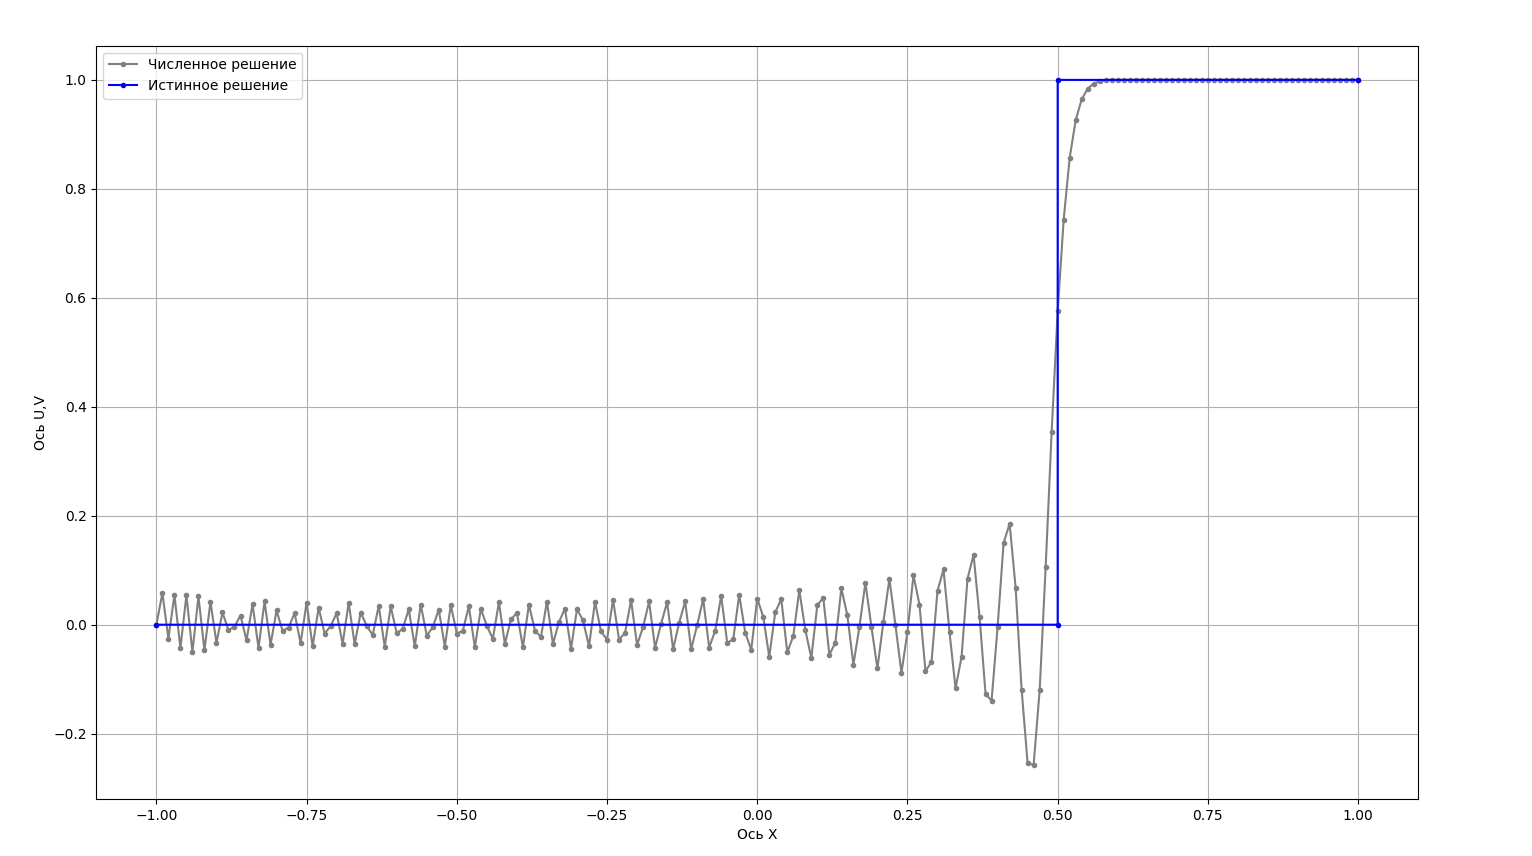
\includegraphics[width=1\linewidth]{Figure_3.png}
    \end{minipage}
    \hfill
    \begin{minipage}[h]{0.5\linewidth}
    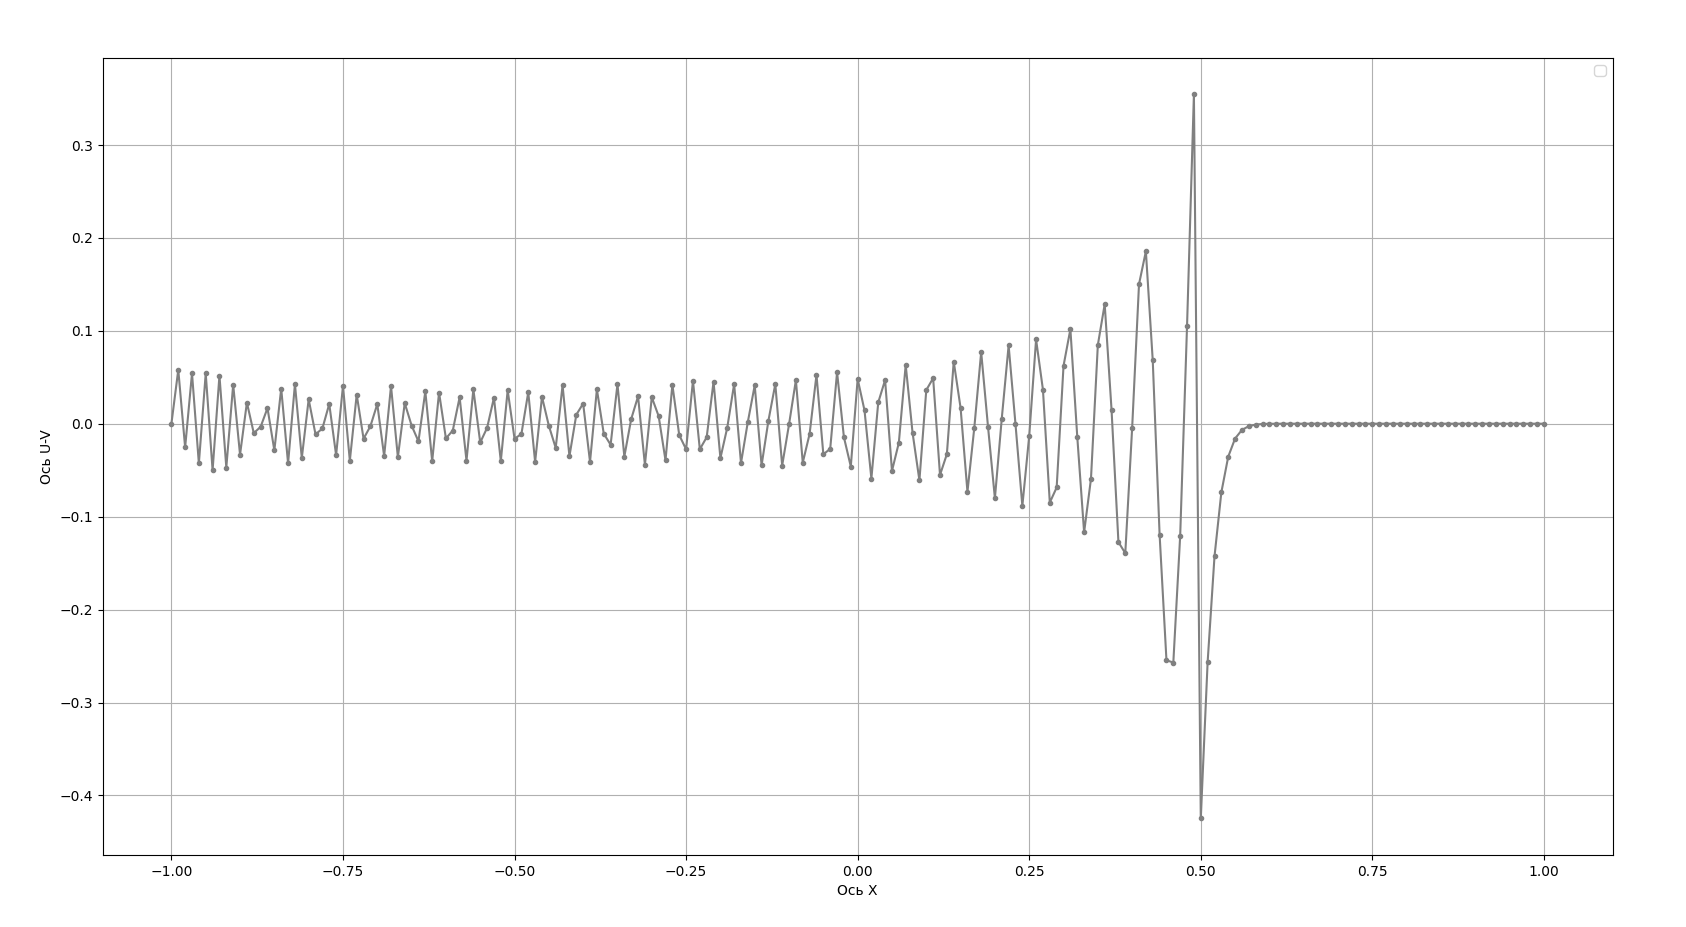
\includegraphics[width=1\linewidth]{Figure_4.png}
    \end{minipage}
    \hfill
    \end{center}
\end{figure}



\section{Нелинейная задача.}
Итак, решаем $v_t+vv_x=0$ в области $Q_T=\{(t,x)|0<t\leqslant 1, -1\leqslant x\leqslant 1 \}$. Граничные условия $v_0(x)=\left\{
\begin{array}{l}
        $0 \text{ , если } х \leqslant 0$
        \\
        $1 \text{ , если } х > 0$
\end{array}
\right.$. Из теоретического решения знаем, что граничные условия примут $v(t,1)=1$ ,$v(t,-1)=0$


\subsection{Явная схема.}
\[
    v_m^{(1)}=v_m^n-\frac{\tau}{h}(F^n_{m+1}-F^n_m);\;\; v^{n+1}_m=\frac12\left(v^n_m+v_m^{(1)}-\frac{\tau}{h}(F(v_m^{(1)})-F(v_{m-1}^{(1)}))\right)
\]
из чего получаем разностную схему ($F(v)=\frac{v^2}{2}$)
\[
    S:=\frac{v^{n+1}_m-v^n_m}{\tau}+\frac{(v^n_{m+1})^2-(v^n_m)^2}{4h}+\frac{(v^{(1)}_m)^2-(v^{(1)}_{m-1})^2}{4h}=0
\]


\subsubsection{Аппроксимация}
Используя выражения
\begin{align*}
\begin{array}{l}
    v_m^{n+1}=v+\dot v \tau+\frac{\ddot v}{2} {\tau}^2+\frac{\dddot v}6{\tau}^3+O({\tau}^4)\\
    v_m^n=v\\
    v^n_{m+1}=v+v' h+\frac{v''}2 h^2+\frac{v'''}6 h^3 +O(h^4)\\
    v^n_{m-1}=v-v' h+\frac{v''}2 h^2-\frac{v'''}6 h^3 +O(h^4)\\
    v_m^{(1)}=v_m^n-\frac{\tau}{2h}( (v^n_{m+1})^2-(v^n_m)^2)\\
    v_{m-1}^{(1)}=v_{m-1}^n-\frac{\tau}{2h}((v^n_m)^2-(v^n_{m-1})^2)\\
    \\
    \dot v +vv'=0\\
    \ddot v -2v(v')^2-v^2v''=0
\end{array}
\end{align*}
Получим следующее выражение:
\[
    S=\frac{\tau^2}{6}(3vv'((v')^2+vv'')+\dddot v)+\frac{\tau h}{4}((v')^3+2vv'v'')+\frac{h^2}{6}(3v'v''+vv''')+O(\tau^3+h^3)
\]
Из чего делаем вывод, что порядок аппроксимации равен 2. 
\subsubsection{Численное решение.}
Преобразуем нашу схему к виду:
\[
    v_m^{n+1}=v_m^n-\frac{\nu}{4}( (v^n_{m+1})^2 -(v_m^n)^2)-\frac{\nu}{4}(v_m^n-v_{m-1}^n-\frac{\nu}{2}( (v_{m+1}^n)^2 -2(v^n_m)^2+(v^n_{m-1})^2))(v^n_m+v^n_{m-1}-\frac{\nu}{2}((v^n_{m+1})^2+(v^n_{m-1})^2))
\]
Граничные условия примут вид: $v(t,-1)=0 \Rightarrow v^n_0=0 \;\; \forall\; n \in (0 \div N)$ , $v(t,1)=1 \Rightarrow v^n_{M_h}=0 \;\; \forall\; n \in (0 \div N)$.

Тогда $\{v^{n+1}_m\}$ вычисляются по набору $\{v^{n}_m\}$ согласно выше описанной системе линейных уравнений.

Тогда расчеты дают следующие результаты:
\begin{align*}
\begin{tabular}{|c|c|c|c|c|c|}
    \hline
    \tau & h & \Delta(v)_{C_h} & \Delta(v)_{L_1,h} & \delta(v)_{C_h} & \delta(v)_{L_1,h} \\
    \hline
    0.100 & 0.100 & 8.498309e-01 & 4.534411e-01 & 8.498309e-01 & 4.540809e-01 \\
    \hline
    0.010 & 0.100 & v5.804220e-01 & 2.321695e-01 & 5.804220e-01 & 3.029365e-01 \\
    \hline
    0.001 & 0.100 & 5.674904e-01 & 2.175393e-01 & 5.674904e-01 & 2.901153e-01 \\
    \hline
    0.100 & 0.010 & inf & nan & nan & nan \\
    \hline
    0.010 & 0.010 & 8.872534e-01 & 4.803884e-01 & 8.872534e-01 & 4.880325e-01 \\
    \hline
    0.001 & 0.010 & 7.092497e-01 & 2.648744e-01 & 7.092497e-01 & 3.451246e-01 \\
    \hline
    0.100 & 0.001 & inf & nan & nan & nan \\
    \hline
    0.010 & 0.001 & inf & nan & nan & nan \\
    \hline
    0.001 & 0.001 & 8.895742e-01 & 4.830139e-01 & 8.895742e-01 & 4.911672e-01 \\
    \hline
\end{tabular}
\end{align*}

Теперь рассмотрим случай равномерного дробления сетки, при исходных данных $\tau = 0.1$, $h = 0.1$.
Причем $\tau_k=\frac{\tau}{2^k}$ и $h_k=\frac{h}{2^k}$.  $\Delta(v,v^k)_\alpha=\|v-v^k\|_\alpha$  и  $\delta(v,v^k)_\alpha=\frac{\|v-v^k\|_\alpha}{\|v\|_{\alpha}}$. 
\begin{align*}
\begin{tabular}{|c|c|c|c|c|c|c|}
    \hline
     & \tau_k& h_k & \Delta(v,\cdot)_{C_h} & \Delta(v,\cdot)_{L_1,h} & \delta(v,\cdot)_{C_h} & \delta(v,\cdot)_{L_1,h} \\   
    \hline
    v^1 & 0.050000 & 0.050000 & 3.692220e-01 & 7.059167e-02 & 3.692220e-01 & 7.069128e-02\\ 
    \hline
    v^2 & 0.025000 & 0.025000 & 6.746718e-01 & 1.038319e-01 & 6.746718e-01 & 1.039784e-01\\
    \hline
    v^3 & 0.012500 & 0.012500 & 4.889888e-01 & 8.394065e-02 & 4.889888e-01 & 8.405909e-02\\
    \hline
    v^4 & 0.006250 & 0.006250 & 5.053363e-01 & 8.653917e-02 & 5.053363e-01 & 8.666127e-02\\
    \hline
    u & 0.100 & 0.100 & 8.498309e-01 & 4.534411e-01 & 8.498309e-01 & 4.540809e-01 \\
    \hline    
\end{tabular}
\end{align*}
    
При исходных данных $\tau = 0.01$, $h = 0.01$.
\begin{align*}
\begin{tabular}{|c|c|c|c|c|c|c|}
    \hline
     & \tau_k& h_k & \Delta(v,\cdot)_{C_h} & \Delta(v,\cdot)_{L_1,h} & \delta(v,\cdot)_{C_h} & \delta(v,\cdot)_{L_1,h} \\   
    \hline
    v^1 & 0.005000 & 0.005000 & 4.814581e-01 & 9.148894e-03 & 4.814581e-01 & 9.294473e-03 \\
    \hline
    v^2 & 0.002500 & 0.002500 & 2.711793e-01 & 7.243046e-03 & 2.711793e-01 & 7.358298e-03 \\
    \hline
    v^3 & 0.001250 & 0.001250 & 2.969553e-01 & 7.737691e-03 & 2.969553e-01 & 7.860815e-03 \\
    \hline
    v^4 & 0.000625 & 0.000625 & 2.980227e-01 & 7.748339e-03 & 2.980227e-01 & 7.871632e-03 \\
    \hline
    u & 0.010 & 0.010 & 8.872534e-01 & 4.803884e-01 & 8.872534e-01 & 4.880325e-01 \\    
    \hline
\end{tabular}
\end{align*}

Таким образом имеем следующие графики:
\begin{figure}[h]
    \begin{center}
    \begin{minipage}[h]{0.49\linewidth}
    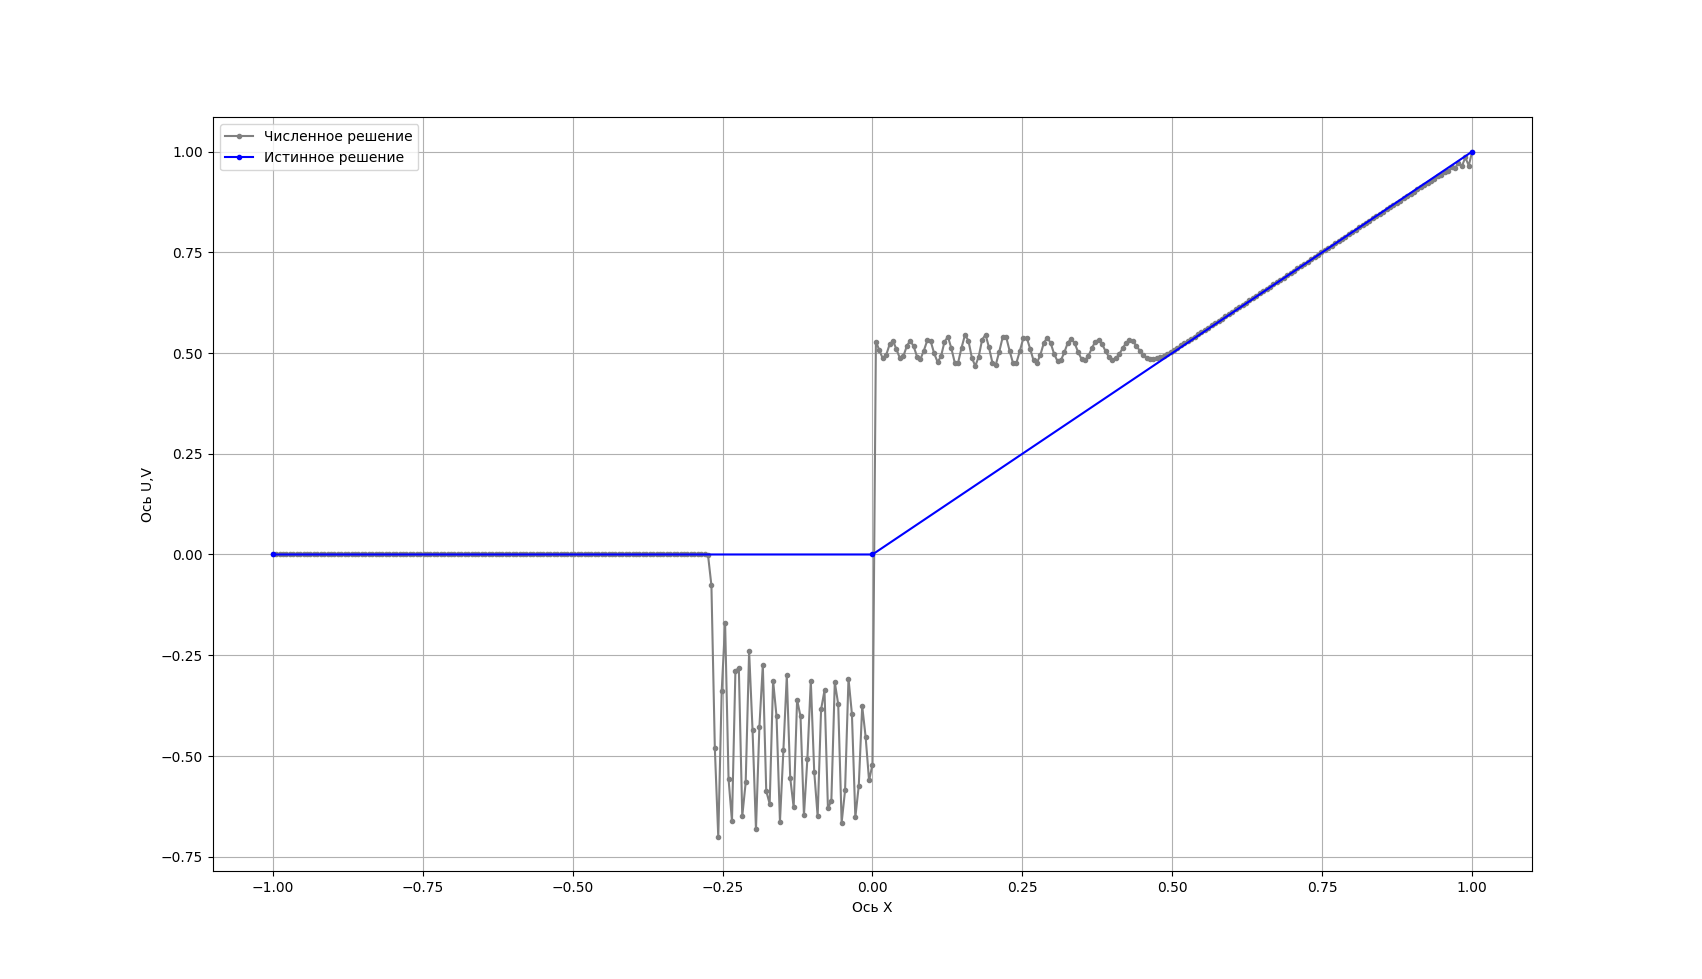
\includegraphics[width=1\linewidth]{Figure_5.png}
    \end{minipage}
    \hfill
    \begin{minipage}[h]{0.5\linewidth}
    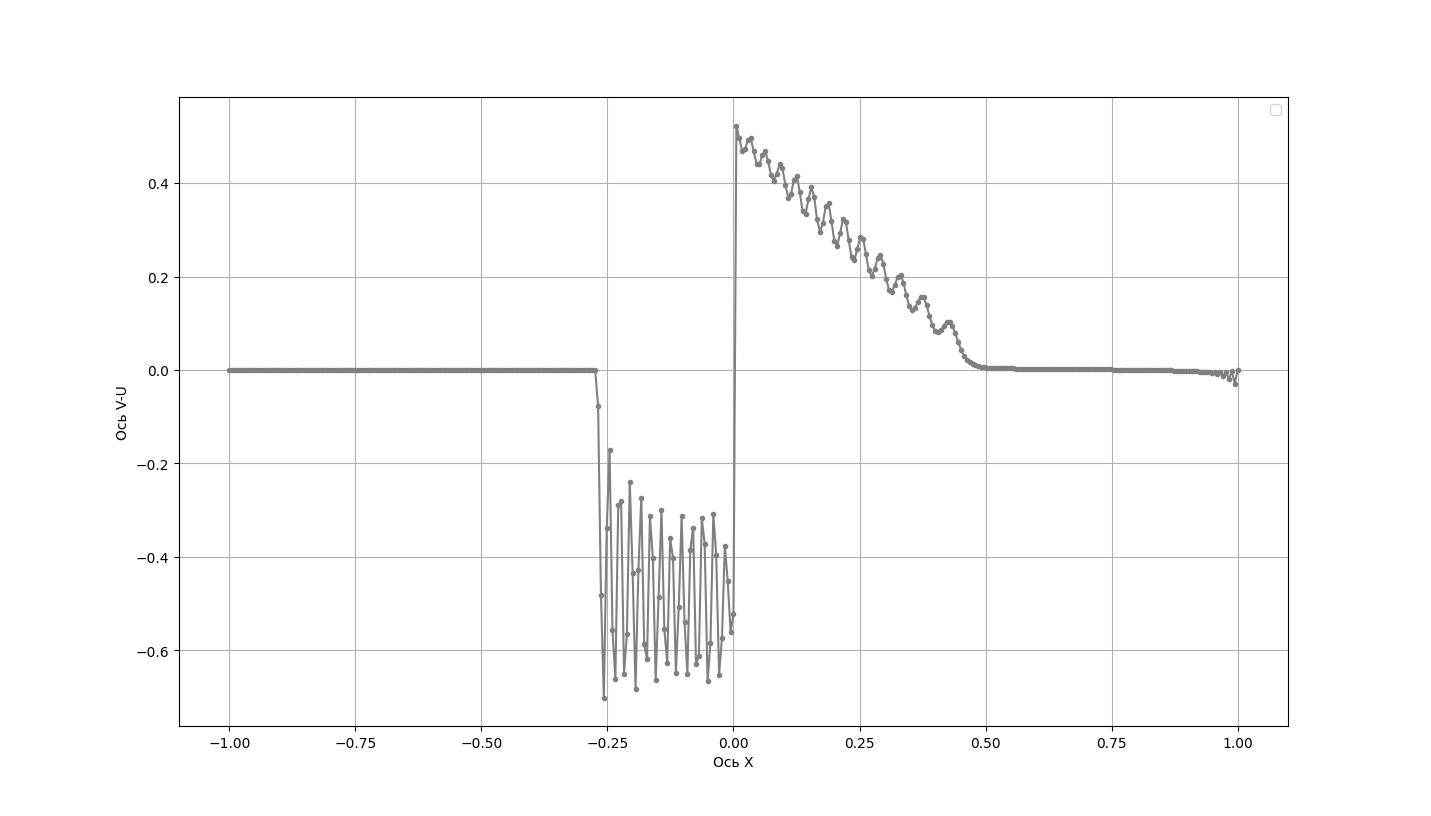
\includegraphics[width=1\linewidth]{Figure_8.png}
    \end{minipage}
    \hfill
    \end{center}
\end{figure}

Видим, что графики показывают решение, отличное от истинного. Пойдем следующим путем, возьмем непрерывные начальные условия вида:
\[
u_0(x)=\left\{
\begin{array}{l}
    0\text{ , при  } x<0 \\
    1\text{ , при  } x>\theta \\
    \frac{x}{\theta}\text{ , при  } 0<x<\theta \\
\end{array}    
\]
Тогда если мы устремим $h\rightarrow0$ , то начальное условие $u_0(x)$ будет сходится к исходному разрывному начальному условию. Так как мы рассматриваем решение в ограниченной области, и это решение определяется характеристиками, которые непрерывно зависят от начальных условий, то и наше решение в области непрерывно зависит от начальных условий. Поэтому решение должно стремится к истинному решению задачи.

Ниже указан результат для шагов $\tau=0.01, \;\; h=0.01$  и уменьшающегося шага $\theta$ (указан на рисунке):
\begin{figure}[h]
    \begin{center}
    \begin{minipage}[h]{0.85\linewidth}
    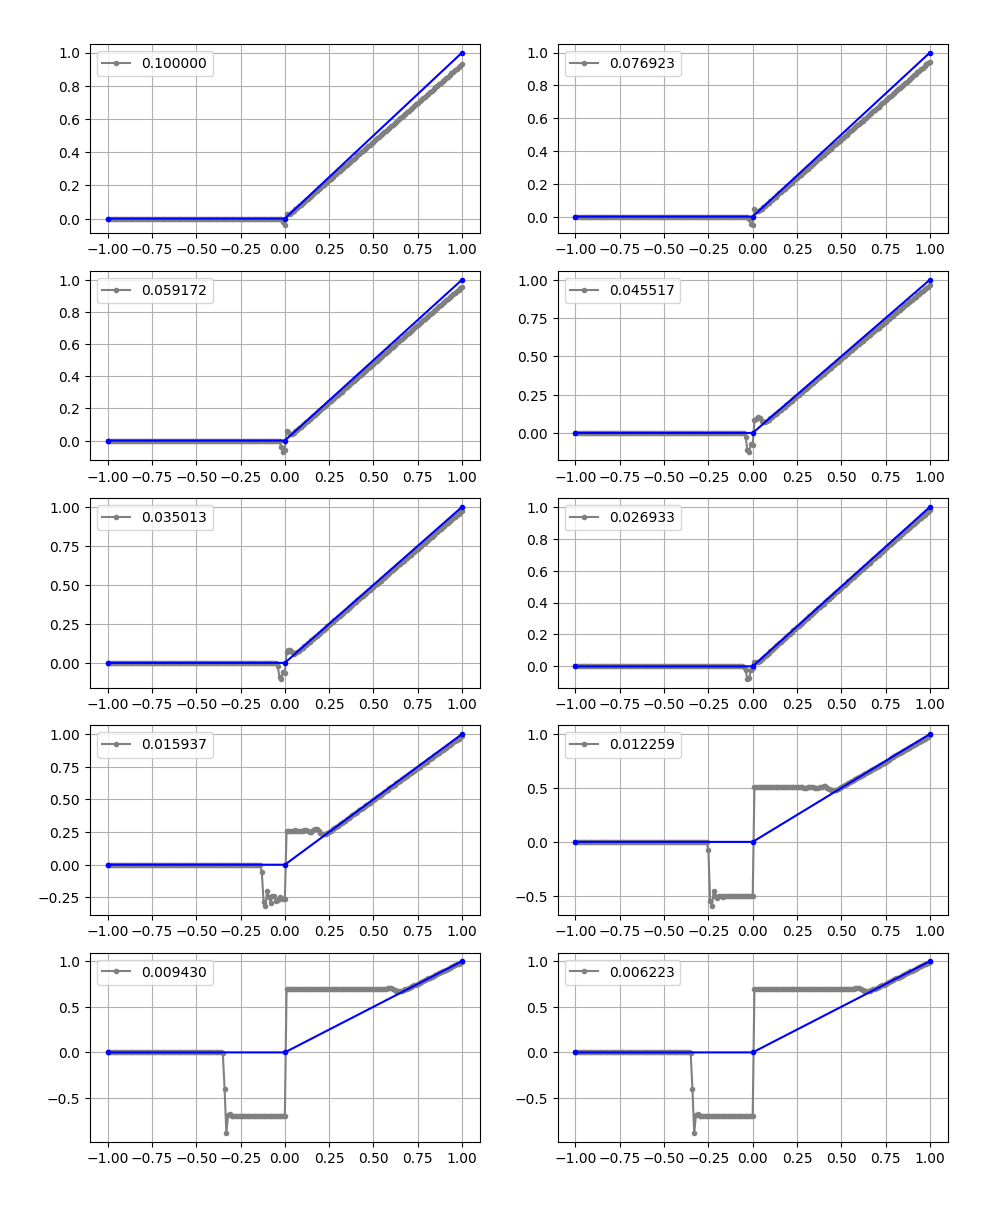
\includegraphics[width=1\linewidth]{Figure_11.png}
    \end{minipage}
    \end{center}
\end{figure}

Видим, что при уменьшении параметра $\theta$ у нуля получаем разрыв. Решением этого становится пропорциональное уменьшение шагов сетки. Например, если в качестве начальных данных взять $ \tau = 0.01 , \;\; h=0.01 , \;\;  \theta =0.1$ , и уменьшать все вдвое, получим следующие данные:
\begin{align*}
    \begin{tabular}{|c|c|c|c|c|c|c|}
        \hline
        \tau & h & \theta  & \Delta(v)_{C_h} & \Delta(v)_{L_1,h} & \delta(v)_{C_h} & \delta(v)_{L_1,h} \\
        \hline
        1.000000e-02 &  1.000000e-02 &  1.000000e-01 &  9.090909e-02  & 4.631973e-02 &  1.000000e-01  & 1.007706e-01 \\
        \hline
        5.000000e-03 &  5.000000e-03 &  5.000000e-02 &  4.761905e-02  & 2.441394e-02  & 5.000000e-02 &  5.094394e-02\\
        \hline
        2.500000e-03 & 2.500000e-03 &  2.500000e-02 &  3.804298e-02  & 1.276872e-02  & 3.899405e-02  & 2.607521e-02 \\
        \hline
        1.250000e-03 &  1.250000e-03 &  1.250000e-02 &  3.917822e-02  & 6.783361e-03  & 3.966795e-02  & 1.370053e-02 \\
        \hline
        6.250000e-04 &  6.250000e-04 &  6.250000e-03 &  3.595207e-02  & 3.733617e-03  & 3.617677e-02  & 7.499207e-03 \\
        \hline
        3.125000e-04 &  3.125000e-04 &  3.125000e-03 &  3.477184e-02  & 2.198689e-03  & 3.488051e-02  & 4.403913e-03 \\
        \hline
        1.562500e-04 &  1.562500e-04 &  1.562500e-03 &  3.480186e-02 &  1.427949e-03  & 3.485624e-02  & 2.856152e-03 \\
        \hline
        7.812500e-05 &  7.812500e-05 &  7.812500e-04 &  3.444687e-02 &  1.042245e-03  & 3.447378e-02  & 2.083217e-03 \\
        \hline
        3.906250e-05 &  3.906250e-05 &  3.906250e-04 &  3.413119e-02 &  8.491674e-04 &  3.414452e-02 &  1.696704e-03 \\
        \hline
        1.953125e-05 &1.953125e-05 &1.953125e-04& 3.379066e-02& 7.525779e-04& 3.379726e-02 &1.503447e-03\\
        \hline
    \end{tabular}
    \end{align*}
    
    Тогда уже для данных  последней строки таблицы имеем график:
    \begin{figure}[h]
        \begin{center}
        \begin{minipage}[h]{0.85\linewidth}
        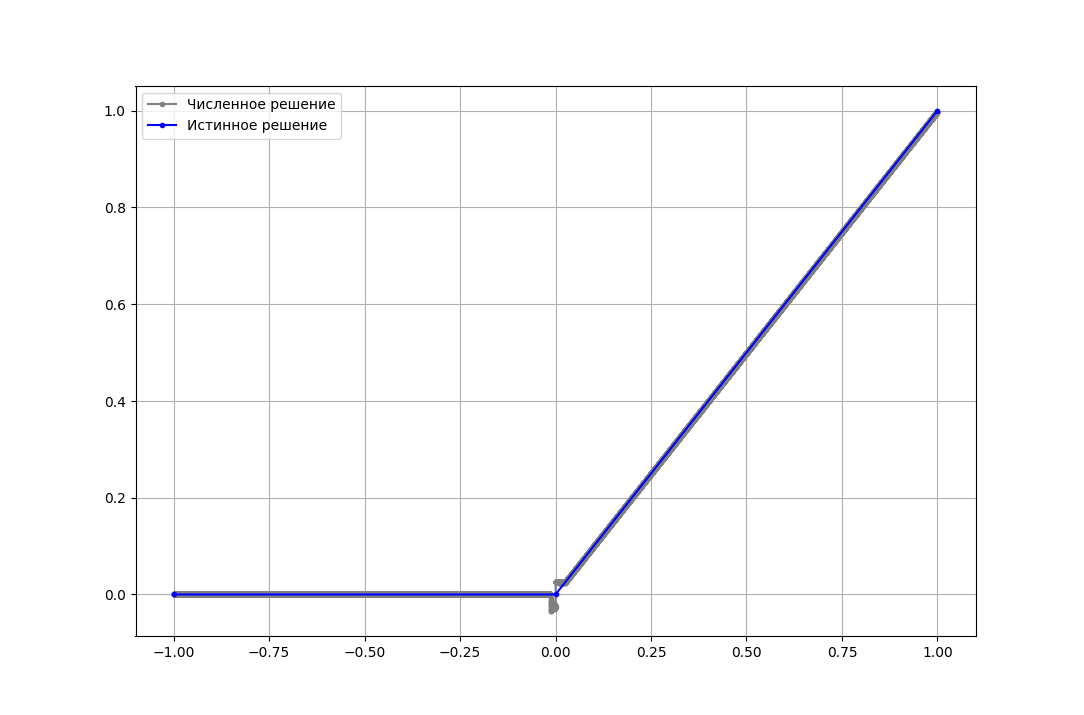
\includegraphics[width=1\linewidth]{Figure_12.png}
        \end{minipage}
        \end{center}
    \end{figure}
    
    Как ниже будет показано, схема обладает устойчивостью, поэтому приведем таблицу , где для фиксированного  $\theta$ показаны результаты уменьшения шага ( выберем $\theta = 0.001$, чтобы иметь достаточное приближение к начальным условиям, но и чтобы не было необходимости работы с очень мелким разбиением сетки):
    \begin{align*}
        \begin{tabular}{|c|c|c|c|c|c|}
            \hline
            \tau & h & \Delta(v)_{C_h} & \Delta(v)_{L_1,h} & \delta(v)_{C_h} & \delta(v)_{L_1,h} \\
            \hline
            1.000000e-04 & 1.000000e-04 & 3.491224e-02 & 1.150314e-03 & 3.494715e-02 & 2.299675e-03 \\
            \hline
            6.896552e-05 & 6.896552e-05 & 2.345893e-02 & 8.057257e-04 & 2.348239e-02 & 1.611958e-03 \\
            \hline
            4.756243e-05 & 4.756243e-05 & 1.659960e-02 & 6.434882e-04 & 1.661620e-02 & 1.287827e-03 \\
            \hline
            3.280194e-05 & 3.280194e-05 & 1.147719e-02 & 5.676639e-04 & 1.148867e-02 & 1.136270e-03 \\
            \hline
            2.262239e-05 & 2.262213e-05 & 9.990010e-04 & 4.995020e-04 & 1.000000e-03 & 9.999802e-04 \\
            \hline
            1.560184e-05 & 1.560148e-05 & 1.000303e-03 & 4.995063e-04 & 1.001303e-03 & 9.999958e-04 \\
            \hline
            1.075998e-05 & 1.075969e-05 & 1.001043e-03 & 4.995036e-04 & 1.002044e-03 & 9.999953e-04 \\
            \hline
            7.420710e-06 & 7.420489e-06 & 2.824629e-03 & 5.029432e-04 & 2.827454e-03 & 1.006878e-03 \\
            \hline
            5.117733e-06 & 5.117589e-06 & 9.990010e-04 & 4.995020e-04 & 1.000000e-03 & 9.999979e-04 \\
            \hline
        \end{tabular}
    \end{align*}

    \begin{align*}
        \begin{tabular}{|c|c|c|c|c|c|c|}
            \hline
            \theta & \tau & h & \Delta(v)_{C_h} & \Delta(v)_{L_1,h} & \delta(v)_{C_h} & \delta(v)_{L_1,h} \\
            \hline
            & 0.010 & 0.010 & 8.872534e-01 & 4.804875e-01 & 8.961259e-01 & 4.881822e-01 \\
            \cline{2-7}
            & 0.001 & 0.010 & 7.092497e-01 & 2.649560e-01 & 7.163422e-01 & 3.452676e-01 \\
            \cline{2-7}
            & 0.0001 & 0.010 & 7.831323e-01 & 2.507228e-01 & 7.909636e-01 & 3.329498e-01 \\
            \cline{2-7}
            & 0.010 & 0.001 & inf & nan & nan & nan \\
            \cline{2-7}
            0.01& 0.001 & 0.001 & 3.876085e-02 & 5.560928e-03 & 3.914846e-02 & 1.120687e-02 \\
            \cline{2-7}
            & 0.0001 & 0.001 & 2.220997e-02 & 5.024782e-03 & 2.243207e-02 & 1.013466e-02 \\
            \cline{2-7}
            & 0.010 & 0.0001 & inf & nan & nan & nan \\
            \cline{2-7}
            & 0.001 & 0.0001 & inf & nan & nan & nan \\
            \cline{2-7}
            & 0.0001 & 0.0001 & 9.900990e-03 & 4.956962e-03 & 1.000000e-02 & 1.001194e-02 \\
            \hline
            & 0.010 & 0.010 & 8.872534e-01 & 4.803984e-01 & 8.881407e-01 & 4.880476e-01 \\
            \cline{2-7}
            & 0.001 & 0.010 & 7.092497e-01 & 2.648844e-01 & 7.099590e-01 & 3.451421e-01 \\
            \cline{2-7}
            & 0.0001 & 0.010 & 7.831323e-01 & 2.506540e-01 & 7.839154e-01 & 3.328281e-01 \\
            \cline{2-7}
            & 0.010 & 0.001 & inf & nan & nan & nan \\
            \cline{2-7}
            0.001& 0.001 & 0.001 & 8.895742e-01 & 4.830149e-01 & 8.904638e-01 & 4.911687e-01 \\
            \cline{2-7}
            & 0.0001 & 0.001 & 6.797345e-01 & 2.674826e-01 & 6.804142e-01 & 3.484362e-01 \\
            \cline{2-7}
            & 0.010 & 0.0001 & inf & nan & nan & nan \\
            \cline{2-7}
            & 0.001 & 0.0001 & inf & nan & nan & nan \\
            \cline{2-7}
            & 0.0001 & 0.0001 & 3.491224e-02 & 1.150314e-03 & 3.494715e-02 & 2.299675e-03 \\
            \hline
            & 0.010 & 0.010 & 8.872534e-01 & 4.803894e-01 & 8.873421e-01 & 4.880340e-01 \\
            \cline{2-7}
            & 0.001 & 0.010 & 7.092497e-01 & 2.648754e-01 & 7.093206e-01 & 3.451263e-01 \\
            \cline{2-7}
            & 0.0001 & 0.010 & 7.831323e-01 & 2.506453e-01 & 7.832106e-01 & 3.328126e-01 \\
            \cline{2-7}
            & 0.010 & 0.001 & inf & nan & nan & nan \\
            \cline{2-7}
            0.0001& 0.001 & 0.001 & 8.895742e-01 & 4.830140e-01 & 8.896631e-01 & 4.911673e-01 \\
            \cline{2-7}
            & 0.0001 & 0.001 & 6.797345e-01 & 2.674819e-01 & 6.798025e-01 & 3.484349e-01 \\
            \cline{2-7}
            & 0.010 & 0.0001 & inf & nan & nan & nan \\
            \cline{2-7}
            & 0.001 & 0.0001 & inf & nan & nan & nan \\
            \cline{2-7}
            & 0.0001 & 0.0001 & 8.419044e-01 & 4.832747e-01 & 8.419886e-01 & 4.914759e-01 \\
            \hline
        \end{tabular}
    \end{align*}


\subsubsection{Устойчивость}

Воспользуемся методом замороженных коэффициентов. Схема имеет вид:
\[
    v^{n+1}_m=v^n_m-\frac{\tau}{2h}(F(v^n_{m+1})-F(v^n_m))-\frac{\tau}{2h}(F(v^{(1)}_m)-F(v^{(1)}_{m-1}))
\]
Запишем это уравнение в вариациях, получим:
\[
    \delta^{n+1}_m=\delta_m^n-\frac{\tau}{2h}(v^n_{m+1}\delta^n_{m+1}-v^n_m\delta^n_m)-\frac{\tau}{2h}(v^{(1)}_m\delta^{(1)}_m-v^{(1)}_{m-1}\delta^{(1)}_{m-1})
\]
Учитывая, что 
\begin{align*}
\begin{array}{l}
    \delta^{(1)}_m=\delta^{n}_m-\frac{\tau}{h}(v^n_{m+1}\delta^n_{m+1}-v^n_m\delta^n_m)\\
    \\
    \delta^{(1)}_{m-1}=\delta^{n}_{m-1}-\frac{\tau}{h}(v^n_{m}\delta^n_{m}-v^n_{m-1}\delta^n_{m-1})\\
    \\
    v^{(1)}_{m-1}=v^n_m+O(\tau+h)=a+O(\tau+h) \; ; \; v^{(1)}_{m} =v^n_m+O(\tau+h)=a+O(\tau+h) \\
    \\
    v^n_{m-1}v^n_m+O(\tau+h)=a+O(\tau+h)   \; ; \;   v^n_m=a    \; ; \;   v^n_{m+1}v^n_m+O(\tau+h)=a+O(\tau+h)\\
\end{array}
\end{align*}
имеем ($\nu=\frac{\tau}{h}$)
\[
    \delta^{n+1}_m=\delta_m^n-\frac{\nu a}{2}(\delta^n_{m+1}-\delta^n_m)-\frac{\nu^2 a^2}{2}(\delta^{n}_{m+1}-2\delta^{n}_{m}+\delta^{n}_{m-1})
\]
Тогда
\[
    \lambda=1+\nu^2 a^2 (\cos{\varphi}-1)-\nu a \sin{\varphi} \cdot i = x+y\cdot i \Rightarrow  
\]
\[
\left(\frac{x-1+\nu^2 a^2}{\nu^2 a^2}\right)^2+\left(\frac{y^2}{\nu a}\right)^2=1
\]
Как минимум требуем, чтобы $\nu^2 a^2 \leqslant 1$ , иначе эллипс лежит вне единичного круга, и условие спектральной устойчивости заведомо не будет выполнено. Тогда, как и в линейной задаче, из геометричесских свойств эллипса и окружности, чтобы эллипс целиком лежал в единичном круге, достаточно того, что в точке касания эллипса и окружности, эллипс оказался "вогнутее" окружности. Выразим для этого правые половины фигур, как функции переменной $y$ ($x_1(y)$ - окружность, $x_2(y)$ - эллипс.),  и разложим их в ряд Тейлора в нуле. Получим: 

$
x_1(y)=1-\frac{y^2}{2}-\frac{y^4}{8}+O(y^6) ,
$

$
x_2(y)=1-\frac{y^2}{2}-\frac{y^4}{8 \; \nu^2 a^2}+O(y^6).
$ 

Откуда видно, что при $\nu^2 a^2 \leqslant 1$ желаемое выполнено, то есть имеем условную сходимость.
\subsection{Неявная схема.}
\[
   S:=v_t+\frac12 (F(\hat{v}))_x+\frac12 (F(v))_\overline{x}=0 
\]
Схема примет вид $(F(v)=\frac{v^2}{2})$:
\[
S=\frac{v^{n+1}_m-v^n_m}{\tau}+\frac{(v^{n+1}_{m+1})^2-(v^{n+1}_m)^2}{4h}+\frac{(v^n_m)^2-(v^n_{m-1})^2}{4h}=0
\]

\subsubsection{Аппроксимация}
Используя выражения
\begin{align*}
\begin{array}{l}
    v_m^{n+1}=v+\dot v \tau+\frac{\ddot v}{2} {\tau}^2+\frac{\dddot v}6{\tau}^3+O({\tau}^4)\\
    v_m^n=v\\
    v^n_{m-1}=v-v' h+\frac{v''}2 h^2-\frac{v'''}6 h^3 +O(h^4)\\
    v^{n+1}_{m+1}=v+\dot v \tau +v' h +\frac{\ddot v}{2} \tau^2 + \dot v' \tau h + \frac{v''}{2} h^2 + \frac{\dddot v}{6} \tau^3 + \frac{\ddot v'}{2} \tau^2 h +\frac{\dot v''}{2}\tau h^2+\frac{v'''}{6} h^3+ O(h^4+\tau^4)   \\
    \\
    \dot v +vv'=0\\
    \ddot v +v'\dot v+v\dot v'=0
\end{array}
\end{align*}
Получим 
\[
 S=-\frac{\dddot v}{12}\tau^2-\frac{\ddot v'}{4}\tau h -\frac{\dot v''}{6} h^2 +O(h^3+ \tau^3)
\]
Получили, что порядок апроксимации равен 2-ум.

\subsubsection{Численное решение.}
Преобразуем нашу схему в виде:
\[
    (v_m^{n+1})^2-\frac{4}{\nu}v^{n+1}_m+\frac{4}{\nu}v_m^n-((v_m^n)^2-(v^n_{m-1})^2+(v^{n+1}_{m+1})^2)=0
\]
Граничные условия примут вид: $v(t,-1)=0 \Rightarrow v^n_0=0 \;\; \forall\; n \in (0 \div N)$ , $v(t,1)=1 \Rightarrow v^n_{M_h}=0 \;\; \forall\; n \in (0 \div N)$.

Согласно шаблону, мы используем в нашей схеме набор точек: $\{(n,m)\; ,\; (n,m-1)\; , \; (n+1,m) \; , \; (n+1,m+1)\}$. Но из граничных условий мы для крайнего положения знаем значение в точке $(n+1,M_h)$, и тогда по схеме можем получить значение в точке $(n+1,M_h-1)$ как решение выше описанного квадратного уравнения. Аналогичные рассуждения проведем для точки $(n+1,M_h-2)$, и так далее итеративно рассчитаем весь ряд.

Остается решить проблему, какой корень выбрать. Пусть $v^n_m=v$, считаем $v_{m+1}^{n+1}=v + O(\tau) + O(h),\;\;v^n_{m-1}=v+O(h),\;\; v^n_m=v$. Из соображений непрерывности решения, потребуем, чтобы корень квадратного уравнения имел вид: $v+O(\tau)+O(h)$.
\[
    \frac{D}4=\frac{4}{\nu^2}-\frac{4}{\nu}\; v+v^2+O(\tau)+O(h)=\left(\frac2\nu -v\right)^2+O(\tau)+O(h) \Rightarrow
\]
\[
    v^{n+1}_m=\frac{2}{\nu}\pm\sqrt{\left(\frac2\nu -v\right)^2+O(\tau)+O(h)}=\frac{2}{\nu} \pm \left|\left(\frac2\nu -v\right)\right|+O(\tau)+O(h)
\]
Поэтому корень будем выбирать по принципу:

\left\{
\begin{array}{l}
    $v^{n+1}_m=\frac{2}{\nu}-\sqrt{\frac{D}4}=\frac{2}{\nu}-\sqrt{\frac{4}{\nu^2}-\frac{4}{\nu}v_m^n+((v_m^n)^2-(v^n_{m-1})^2+(v^{n+1}_{m+1})^2)}\text{,  если  }\frac2\nu -v^n_m \geqslant 0 $\\
    $v^{n+1}_m=\frac{2}{\nu}+\sqrt{\frac{D}4}=\frac{2}{\nu}+\sqrt{\frac{4}{\nu^2}-\frac{4}{\nu}v_m^n+((v_m^n)^2-(v^n_{m-1})^2+(v^{n+1}_{m+1})^2)}\text{,  если  }\frac2\nu -v^n_m \leqslant 0 $
\end{array}
\right.

Тогда  $\{v^{n+1}_m\}$ рассчитаем по набору $\{v^{n}_m\}$ согласно выше описанной системе линейных уравнений.

Расчеты дают следующие результаты:
\begin{align*}
\begin{tabular}{|c|c|c|c|c|c|}
    \hline
    \tau & h & \Delta(v)_{C_h} & \Delta(v)_{L_1,h} & \delta(v)_{C_h} & \delta(v)_{L_1,h} \\
    \hline
    0.100 & 0.100 & 4.768202e-01 & 3.155235e-01 & 4.768202e-01 & 5.575204e-01 \\
    \hline
    0.010 & 0.100 & 5.370815e-01 & 4.315899e-01 & 5.370815e-01 & 5.980116e-01 \\
    \hline
    0.001 & 0.100 & 5.623037e-01 & 4.515290e-01 & 5.623037e-01 & 6.058267e-01 \\
    \hline
    0.100 & 0.010 & 1.371363e+00 & 9.600960e-01 & 1.000000e+00 & 6.575568e-01 \\
    \hline
    0.010 & 0.010 & 4.980405e-01 & 3.140581e-01 & 4.980405e-01 & 5.576327e-01 \\
    \hline
    0.001 & 0.010 & 7.605155e-01 & 4.717831e-01 & 7.605155e-01 & 6.502340e-01 \\
    \hline
    0.100 & 0.001 & 1.391977e+00 & 9.932151e-01 & 1.000000e+00 & 6.651521e-01 \\
    \hline
    0.010 & 0.001 & 1.464911e+00 & 9.212901e-01 & 1.000000e+00 & 6.482069e-01 \\
    \hline
    0.000 & 0.000 & 4.999803e-01 & 3.125607e-01 & 4.999803e-01 & 5.556130e-01 \\
    \hline
\end{tabular}
\end{align*}

Теперь рассмотрим случай равномерного дробления сетки, при исходных данных $\tau = 0.1$, $h = 0.1$.
Причем $\tau_k=\frac{\tau}{2^k}$ и $h_k=\frac{h}{2^k}$.  $\Delta(v,v^k)_\alpha=\|v-v^k\|_\alpha$  и  $\delta(v,v^k)_\alpha=\frac{\|v-v^k\|_\alpha}{\|v\|_{\alpha}}$. 
\begin{align*}
\begin{tabular}{|c|c|c|c|c|c|c|}
    \hline
     & \tau_k& h_k & \Delta(v,\cdot)_{C_h} & \Delta(v,\cdot)_{L_1,h} & \delta(v,\cdot)_{C_h} & \delta(v,\cdot)_{L_1,h} \\   
    \hline
    v^1 & 0.050000 & 0.050000 & 1.302024e-01 & 4.675061e-02 & 1.302024e-01 & 8.260689e-02 \\ 
    \hline
    v^2 & 0.025000 & 0.025000 & 3.074147e+00 & 2.332509e+00 & 3.074147e+00 & 4.121472e+00 \\
    \hline
    v^3 & 0.012500 & 0.012500 & 2.935753e+00 & 2.719528e+00 & 2.935753e+00 & 4.805321e+00 \\
    \hline
    v^4 & 0.006250 & 0.006250 & 2.986898e+00 & 2.606632e+00 & 2.986898e+00 & 4.605837e+00 \\
    \hline
    u & 0.010 & 0.010 & 4.980405e-01 & 3.140581e-01 & 4.980405e-01 & 5.576327e-01 \\
    \hline
\end{tabular}
\end{align*}
    
При исходных данных $\tau = 0.01$, $h = 0.01$.
\begin{align*}
\begin{tabular}{|c|c|c|c|c|c|c|}
    \hline
     & \tau_k& h_k & \Delta(v,\cdot)_{C_h} & \Delta(v,\cdot)_{L_1,h} & \delta(v,\cdot)_{C_h} & \delta(v,\cdot)_{L_1,h} \\   
    \hline
    v^1 & 0.005000 & 0.005000 & 3.162270e+00 & 2.347001e+00 & 3.162270e+00 & 4.167270e+00 \\
    \hline
    v^2 & 0.002500 & 0.002500 & 3.866018e+00 & 2.317555e+00 & 3.866018e+00 & 4.114986e+00 \\
    \hline
    v^3 & 0.001250 & 0.001250 & 2.928915e+00 & 2.235609e+00 & 2.928915e+00 & 3.969485e+00 \\
    \hline
    v^4 & 0.000625 & 0.000625 & 3.115215e+00 & 2.345264e+00 & 3.115215e+00 & 4.164184e+00 \\
    \hline
    u & 0.010 & 0.010 & 4.980405e-01 & 3.140581e-01 & 4.980405e-01 & 5.576327e-01 \\
    \hline
\end{tabular}
\end{align*}

\newpage
Таким образом имеем следующие графики:
\begin{figure}[h]
    \begin{center}
    \begin{minipage}[h]{0.49\linewidth}
    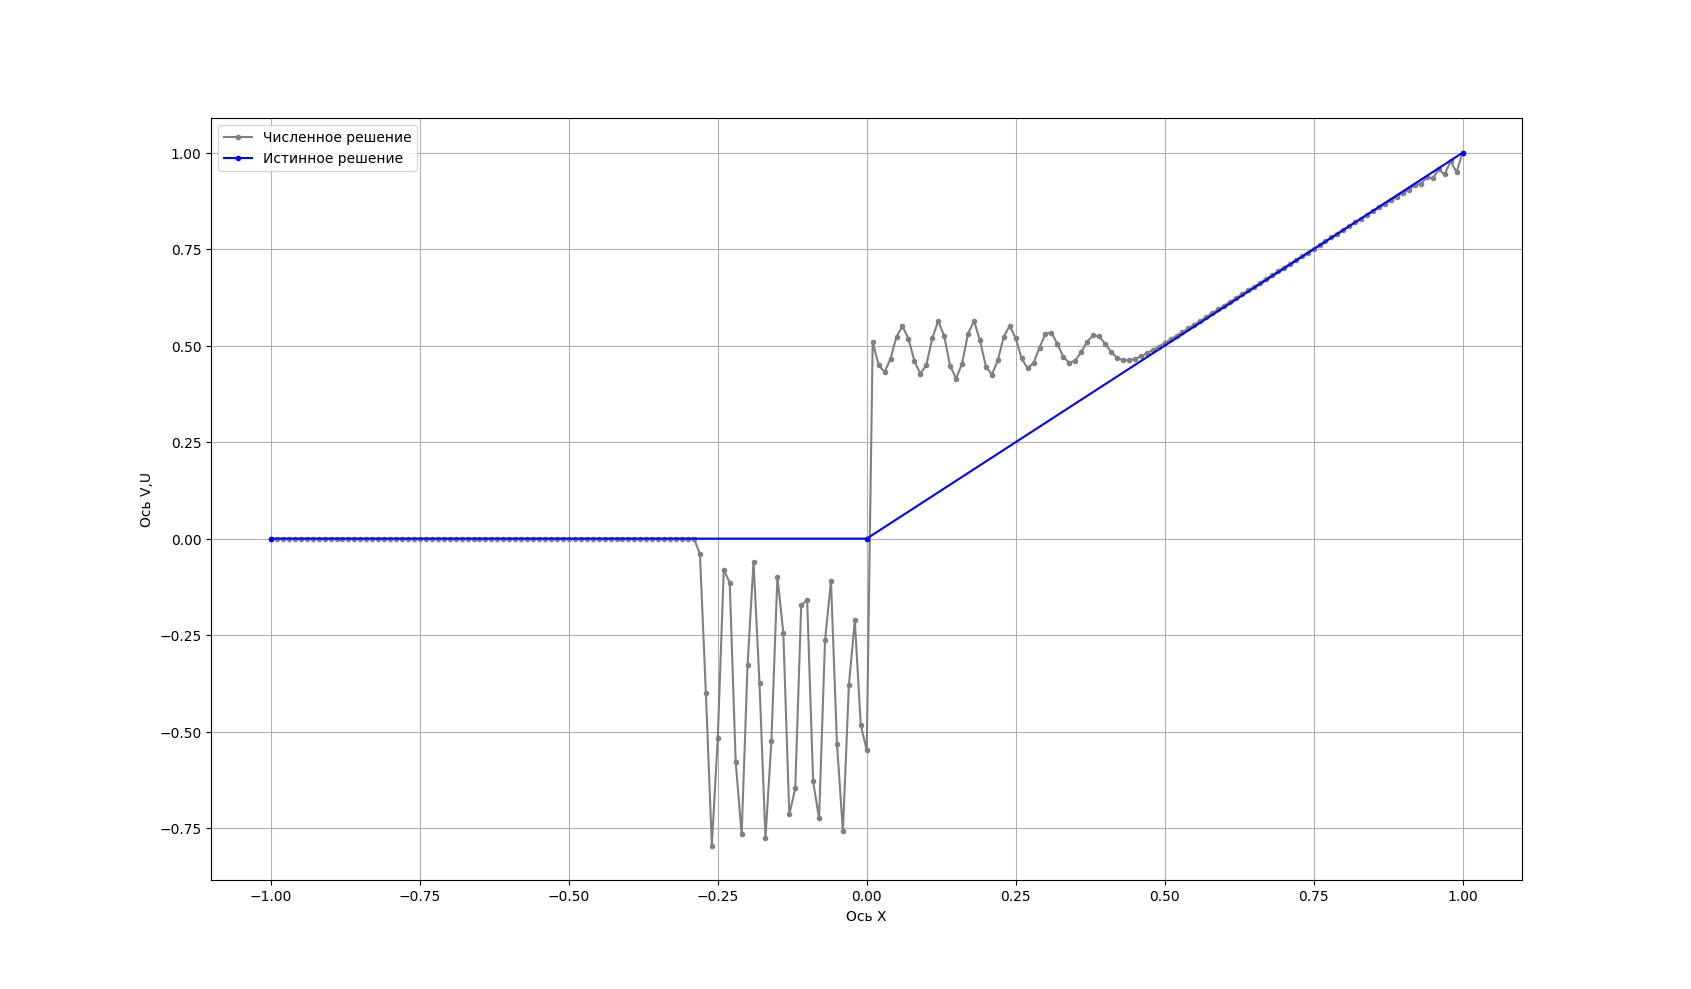
\includegraphics[width=1\linewidth]{Figure_9.png}
    \end{minipage}
    \hfill
    \begin{minipage}[h]{0.5\linewidth}
    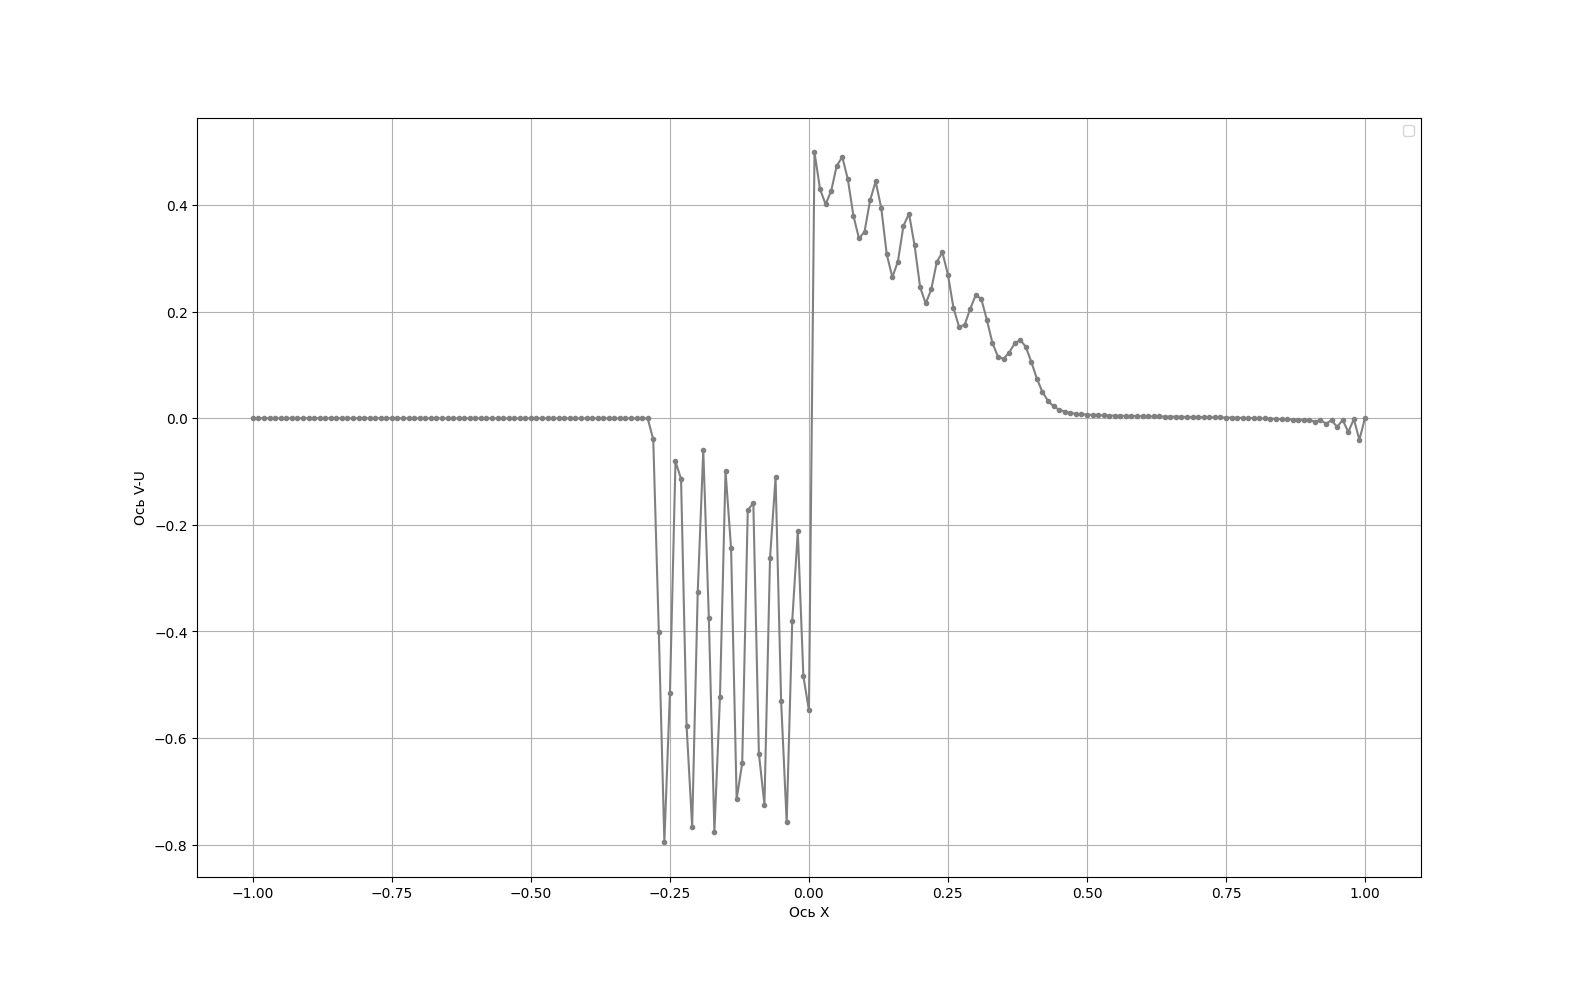
\includegraphics[width=1\linewidth]{Figure_10.png}
    \end{minipage}
    \hfill
    \end{center}
\end{figure}

Также, как и с задачей выше, перейдем к непрерывной постановке. C учетом того, что шаги должны уменьшатся пропорционально параметру $\theta$, получим следующую таблицу:
\begin{align*}
    \begin{tabular}{|c|c|c|c|c|c|c|}
        \hline
        \tau & h & \theta  & \Delta(v)_{C_h} & \Delta(v)_{L_1,h} & \delta(v)_{C_h} & \delta(v)_{L_1,h} \\
        \hline
        1.000000e-02 & 1.000000e-02 & 2.000000e-01 & 5.748999e-01 & 2.918486e-01 & 6.898799e-01 & 6.930964e-01 \\ 
        \hline
        5.000000e-03 & 5.000000e-03 & 1.000000e-01 & 5.408532e-01 & 2.728740e-01 & 5.949385e-01 & 5.971017e-01 \\
        \hline
        2.500000e-03 & 2.500000e-03 & 5.000000e-02 & 5.213990e-01 & 2.620570e-01 & 5.474690e-01 & 5.487538e-01 \\
        \hline
        1.250000e-03 & 1.250000e-03 & 2.500000e-02 & 5.109604e-01 & 2.562514e-01 & 5.237344e-01 & 5.244858e-01 \\
        \hline
        6.250000e-04 & 6.250000e-04 & 1.250000e-02 & 5.055478e-01 & 2.532426e-01 & 5.118672e-01 & 5.123300e-01 \\
        \hline
        3.125000e-04 & 3.125000e-04 & 6.250000e-03 & 5.027912e-01 & 2.517082e-01 & 5.059336e-01 & 5.062443e-01 \\
        \hline
        1.562500e-04 & 1.562500e-04 & 3.125000e-03 & 5.013999e-01 & 2.509357e-01 & 5.029668e-01 & 5.032017e-01 \\
        \hline
        7.812500e-05 & 7.812500e-05 & 1.562500e-03 & 5.007011e-01 & 2.505466e-01 & 5.014834e-01 & 5.016791e-01 \\
        \hline
    \end{tabular}
    \end{align*}
    
    Тогда уже для данных  последней строки таблицы имеем график:
    \begin{figure}[h]
        \begin{center}
        \begin{minipage}[h]{0.85\linewidth}
        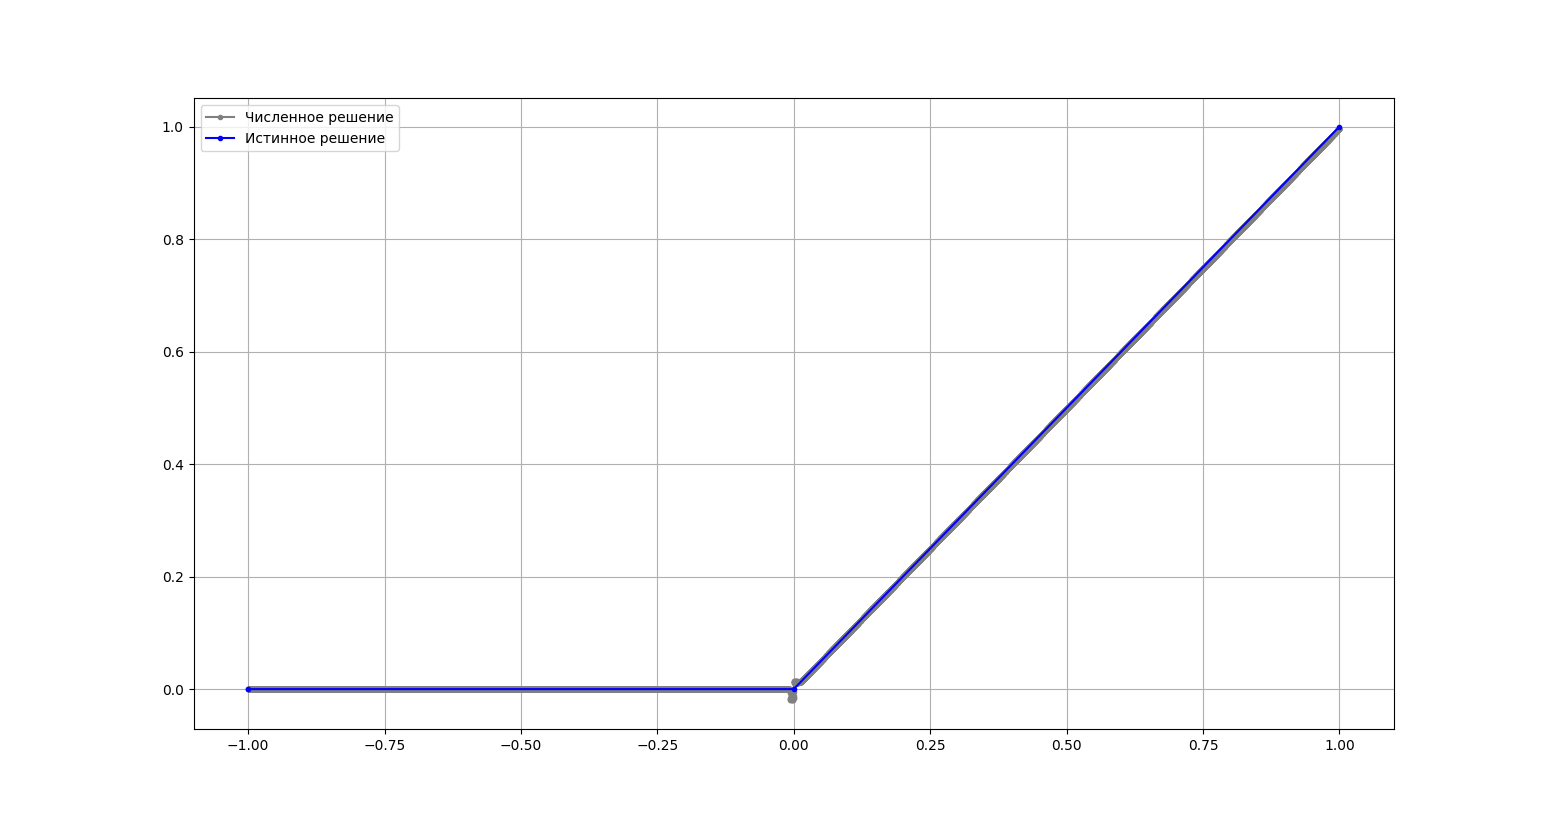
\includegraphics[width=1\linewidth]{Figure_13.png}
        \end{minipage}
        \end{center}
    \end{figure}

    Как ниже будет показано, схема обладает устойчивостью, поэтому приведем таблицу , где для фиксированного  $\theta$ показаны результаты уменьшения шага ( выберем $\theta = 0.001$, чтобы иметь достаточное приближение к начальным условиям, но и чтобы не было необходимости работы с очень мелким разбиением сетки):
    \begin{align*}
        \begin{tabular}{|c|c|c|c|c|c|}
            \hline
            \tau & h & \Delta(v)_{C_h} & \Delta(v)_{L_1,h} & \delta(v)_{C_h} & \delta(v)_{L_1,h} \\
            \hline
            1.000000e-04 & 1.000000e-04 & 5.003971e-01 & 2.508752e-01 & 5.008975e-01 & 5.015727e-01 \\
            \hline
            6.896552e-05 & 6.896552e-05 & 5.004291e-01 & 2.505374e-01 & 5.009295e-01 & 5.012532e-01 \\
            \hline
            4.756243e-05 & 4.756243e-05 & 5.004752e-01 & 2.503914e-01 & 5.009757e-01 & 5.011174e-01 \\
            \hline
            3.280194e-05 & 3.280194e-05 & 5.004992e-01 & 2.503161e-01 & 5.009997e-01 & 5.010500e-01 \\
            \hline
            2.262239e-05 & 2.262213e-05 & 1.284168e+02 & 5.936790e+00 & 1.000000e+00 & 1.091807e+00 \\
            \hline
            1.560184e-05 & 1.560148e-05 & 5.004955e-01 & 2.502498e-01 & 5.009960e-01 & 5.009923e-01 \\
            \hline
            1.075998e-05 & 1.075969e-05 & 4.514705e+02 & 5.579026e+00 & 1.000000e+00 & 1.098354e+00 \\
            \hline
            7.420710e-06 & 7.420489e-06 & 5.004921e-01 & 2.502532e-01 & 5.009926e-01 & 5.009997e-01 \\
            \hline
            5.117733e-06 & 5.117589e-06 & 7.149301e+02 & 5.588583e+00 & 1.000000e+00 & 1.098235e+00 \\
            \hline
        \end{tabular}
    \end{align*}

    \begin{align*}
        \begin{tabular}{|c|c|c|c|c|c|c|}
            \hline
            \theta & \tau & h & \Delta(v)_{C_h} & \Delta(v)_{L_1,h} & \delta(v)_{C_h} & \delta(v)_{L_1,h} \\
            \hline
            & 0.010 & 0.010 & 4.980405e-01 & 3.141079e-01 & 5.030209e-01 & 5.577704e-01 \\
            \cline{2-7}
            & 0.001 & 0.010 & 7.605155e-01 & 4.718589e-01 & 7.681207e-01 & 6.504066e-01 \\
            \cline{2-7}
            & 0.0001 & 0.010 & 7.907147e-01 & 4.937037e-01 & 7.986218e-01 & 6.600859e-01 \\
            \cline{2-7}
            & 0.010 & 0.001 & 2.024141e+00 & 1.025022e+00 & 1.000000e+00 & 1.372072e+00 \\
            \cline{2-7}
            0.1& 0.001 & 0.001 & 5.039357e-01 & 2.530951e-01 & 5.089750e-01 & 5.100903e-01 \\
            \cline{2-7}
            & 0.0001 & 0.001 & 5.038431e-01 & 2.524766e-01 & 5.088815e-01 & 5.093368e-01 \\
            \cline{2-7}
            & 0.010 & 0.0001 & 2.252021e+00 & 1.068472e+00 & 1.000000e+00 & 1.726594e+00 \\
            \cline{2-7}
            & 0.001 & 0.0001 & 1.509266e+01 & 1.310483e+00 & 1.000000e+00 & 1.300448e+00 \\
            \cline{2-7}
            & 0.0001 & 0.0001 & 5.048512e-01 & 2.524815e-01 & 5.098998e-01 & 5.099550e-01 \\
            \hline
            & 0.010 & 0.010 & 4.980405e-01 & 3.140631e-01 & 4.985385e-01 & 5.576466e-01 \\
            \cline{2-7}
            & 0.001 & 0.010 & 7.605155e-01 & 4.717925e-01 & 7.612760e-01 & 6.502556e-01 \\
            \cline{2-7}
            & 0.0001 & 0.010 & 7.907147e-01 & 4.936355e-01 & 7.915054e-01 & 6.599345e-01 \\
            \cline{2-7}
            & 0.010 & 0.001 & 1.464911e+00 & 9.821714e-01 & 1.000000e+00 & 1.363353e+00 \\
            \cline{2-7}
            0.01& 0.001 & 0.001 & 4.998035e-01 & 3.125741e-01 & 5.003033e-01 & 5.557090e-01 \\
            \cline{2-7}
            & 0.0001 & 0.001 & 7.701925e-01 & 4.753552e-01 & 7.709627e-01 & 6.550593e-01 \\
            \cline{2-7}
            & 0.010 & 0.0001 & 1.431703e+00 & 9.901849e-01 & 1.000000e+00 & 1.759950e+00 \\
            \cline{2-7}
            & 0.001 & 0.0001 & 1.772640e+00 & 1.109660e+00 & 1.000000e+00 & 1.364084e+00 \\
            \cline{2-7}
            & 0.0001 & 0.0001 & 5.003971e-01 & 2.508752e-01 & 5.008975e-01 & 5.015727e-01 \\
            \hline
            & 0.010 & 0.010 & 4.980405e-01 & 3.140586e-01 & 4.980903e-01 & 5.576341e-01 \\
            \cline{2-7}
            & 0.001 & 0.010 & 7.605155e-01 & 4.717840e-01 & 7.605916e-01 & 6.502362e-01 \\
            \cline{2-7}
            & 0.000 & 0.010 & 7.907147e-01 & 4.936268e-01 & 7.907937e-01 & 6.599152e-01 \\
            \cline{2-7}
            & 0.010 & 0.001 & 1.464911e+00 & 9.738558e-01 & 1.000000e+00 & 1.336384e+00 \\
            \cline{2-7}
            0.001& 0.001 & 0.001 & 4.998035e-01 & 3.125736e-01 & 4.998534e-01 & 5.557078e-01 \\
            \cline{2-7}
            & 0.000 & 0.001 & 7.701925e-01 & 4.753545e-01 & 7.702695e-01 & 6.550578e-01 \\
            \cline{2-7}
            & 0.010 & 0.0001 & 1.407253e+00 & 9.669379e-01 & 1.000000e+00 & 1.721481e+00 \\
            \cline{2-7}
            & 0.001 & 0.0001 & 1.464911e+00 & 1.012735e+00 & 1.000000e+00 & 1.410059e+00 \\
            \cline{2-7}
            & 0.0001 & 0.0001 & 4.999803e-01 & 3.125608e-01 & 5.000303e-01 & 5.556130e-01 \\ 
            \hline
        \end{tabular}
    \end{align*}

\subsubsection{Устойчисвость}
Проводя аналогичные рассуждения, что и в задаче выше, получаем уравнение в вариациях ($\nu=\frac{\tau}{2h}$):
\[
    \delta^{n+1}_m-\delta^n_m=a \nu (\delta^{n+1}_{m+1}-\delta^{n+1}_m+\delta^n_m-\delta^n_{m-1})
\]
Тогда
\[
    \lambda=\frac{1+a\nu-a\nu e^{- i\varphi}}{1+a\nu-a\nu e^{i\varphi}}=\frac{1+a\nu-a\nu \cos{\varphi} +a\nu \sin{\varphi} \cdot i}{1+a\nu-a\nu \cos{\varphi} - a\nu \sin{\varphi} \cdot i} \;\; \Rightarrow |\lambda|\equiv 1
\]
То есть имеем безусловную устойчивость.
\end{document}
